%
% This work is licensed under a Creative Commons Attribution-ShareAlike 4.0 International License.
%

\documentclass[10pt, a5paper, twoside, openany]{memoir}

\setsecnumdepth{subsection}

\title{Introduction to Fluid Dynamics}
\author{Joseph D. MacMillan}
\date{}


\usepackage{graphicx}
\usepackage{color} 
\usepackage{amsmath, amssymb}
\usepackage{libertinus}
\usepackage{microtype}
\usepackage{layout}
\usepackage[most]{tcolorbox}
\tcbuselibrary{skins,breakable}
\usepackage[hang, small, bf]{caption}
\captionsetup[table]{position=top}
\captionsetup[figure]{position=bottom}
\usepackage[hyphens]{url}
\usepackage[hidelinks]{hyperref}
\hypersetup{pdftitle={Introduction to Fluid Dynamics}}
\hypersetup{pdfauthor={Joseph D. MacMillan}}
\urlstyle{rm}


% Set page margins, etc
\setstocksize{9in}{6in}
\settrimmedsize{\stockheight}{\stockwidth}{*}
\settrims{0pt}{0pt}

\setlxvchars %define lenght 65 char of the used font
\settypeblocksize{*}{1.05\lxvchars}{1.7}
\setbinding{20pt} 
\setlength{\headheight}{30pt}
\setlength{\footskip}{20pt}

\setulmargins{90pt}{*}{*}
\setlrmargins{*}{*}{*}
\setheaderspaces{*}{30pt}{*}

\setmarginnotes{0.01pt}{20pt}{\onelineskip}
\checkandfixthelayout

\setcounter{tocdepth}{3}



\newcommand{\uu}{\symbfup{u}}
\newcommand{\grad}{\symbfup{\nabla}}
\newcommand{\curl}{\symbfup{\nabla} \times}
\newcommand{\dfdx}[2]{\frac{\partial {#1}}{\partial {#2}}}
\newcommand{\ddfdx}[2]{\frac{\partial^2 {#1}}{\partial {#2}^2}}
\newcommand{\vort}{\symbfup{\omega}}
\renewcommand\vec{\symbfup}
\newcommand{\unit}[1]{\hat{\vec{#1}}}
\newcommand{\U}{\mathbb{U}}
\newcommand{\V}{\mathbb{V}}
\newcommand{\LL}{\mathbb{L}^2}
\newcommand{\LLLL}{\mathbb{L}^4}


%\DeclareMathAlphabet{\mathbfsf}{\encodingdefault}{\sfdefault}{bx}{sl}
\newcommand{\tens}[1]{\mathbfsfit{#1}}


\newcounter{example}[chapter]
\def\theexample{\thechapter.\arabic{example}}
\newenvironment{example}[1][ ]{\refstepcounter{example}
\begin{tcolorbox}[breakable, sharp corners, boxrule = 0pt, frame empty, opacityframe=0, parbox=false]
\textbf{Example \theexample \ -- #1.}
}
{ 
\end{tcolorbox}
}

\newenvironment{theorem}[1][ ]{
\begin{tcolorbox}[breakable, sharp corners, boxrule = 0pt, frame empty, opacityframe=0, parbox=false]
\textbf{#1.}
}
{ 
\end{tcolorbox}
}

\newcounter{problem}[chapter]
\def\theproblem{\thechapter.\arabic{problem}}
\newenvironment{problem}[1][ ]{\refstepcounter{problem} \noindent \textbf{Problem \theproblem \ -- #1.}}{\vspace{0.1in}}


\begin{document}

\frontmatter

\maketitle

\begin{center}

\includegraphics[width=\linewidth]{Figures/fig_cover_wave}

\vspace{1in}

{\small

This version was compiled on \today.  For the most up-to-date version and supplementary material, see \href{https://josephmacmillan.github.io/IntroductionToFluidDynamics/index.html}{josephmacmillan.github.io/IntroductionToFluidDynamics}.

\vspace{2in}

This work is licensed under a \href{https://creativecommons.org/licenses/by-sa/4.0/}{Creative Commons Attribution-ShareAlike 4.0 International License}.
}
\end{center}


\newpage

\tableofcontents

\chapter{Preface}

I have to confess right away that I'm not an expert in the subject of fluid dyanmics; I was given an opportunity to teach a course on it a number of years ago and didn't want to refuse, and I assumed my single graduate-level course in fluids was enough preparation.  I'm an astrophysicist by trade, but not one who normally does astrophysical fluid research.  Regardless, I threw myself into the course, and ended up teaching it numerous times, improving my notes each time.  I initially taught from Acheson's very fine \emph{Elementary Fluid Dynamics}, but found it a little too advanced for my students, who were upper undergraduate physics and math students.  Other fluid dynamics textbooks I found were either graduate-level like Acheson's or geared towards engineering and applied fluid mechanics.  So, as all textbooks are created as far as I'm aware, I resolved to turn my binder of notes into a textbook to fit the gap: I wanted a clear, concise, and readable book aimed at upper undergrads in physics and math.  I started it in 2014 or so, but didn't really make any progress until 2022 when I finally had time, in the form of a development leave, to focus on it.  It was a tremendous amount of fun to write.

\section{Who is this book for?}

This is for undergraduate physics and math students interested in solving problems in fluid dynamics.  I assume some basic background -- you, the reader, should have some experience with vector calculus and solving ordinary differential equations -- but even then I'll remind you when necessary what you probably learned in your second year physics and math classes.  Otherwise, I introduce the math when we need it: there's a short section on complex numbers, I spend quite a bit of time going through the process of separation of variables to solve partial difference equations, and topics like Fourier analysis is introduced in the amount we need.

On the other hand, graduate students in physics or math likely won't find enough here to keep them interested beyond the basics -- there's no real discussion of instability or turbulence, or shock waves, or gas dynamics, or other advanced topics, and the amount of time spent on computational methods is much too brief.  Similarly, engineering students likely won't find enough applied work here; the focus is consistently on theory and problem-solving, and many common engineering topics typical in fluid mechanics courses is missing.

To keep things familiar for undergrads, I've used notation from Griffiths' very popular \emph{Introduction to Electrodynamics}, even when not commonly in use in the subject (I use $s$ for the radial coordinate in the cylindrical coordinate system, for example). And I've tried to keep a fairly informal tone throughout the book, so I hope students find it easy to read and not too dense.

\section{What does this book cover?}

The basics of fluid flow as I see them.  That means, after a brief introduction on notation, terms, and visualization, starting with the famous Navier-Stokes equation.  Most students at this point in their career have at least heard of it (and how hard it is to solve!), and solving the first example (Poiseuille flow) is a great introduction to PDEs.  But there's only so much you can do analytically with the Navier-Stokes, so we stop after some basic circular flow examples.  

Then we turn to ideal flows and Euler's equation, and spend a lot of time on incompressible, irrotational flows.  Classic examples like flow past a cylinder are covered, both by solving Lapace's equation but then again in the complex plane with the Milne-Thompson circle theorem.  Conformal mapping is used to handle more complex shapes, and we even discuss a little bit of aerodynamics -- how does an airplane fly?  Ideal line vortexes are used to model vortex pairs and vortex streets.

We end with a basic discussion of small-amplitude surface waves, including both gravity and capillary waves, as well as the classic derivation of sound waves.  The last chapter in the book is devoted to special topics that I deemed too advanced or too adjacent to fit into any of the first five chapters.  It's here that I actually derive the Navier-Stokes equations, talk a little bit about boundary layers, handle the classic dam breaking problem, and derive Stokes law for very viscous flow past a sphere.  I even put a little bit of astrophysics in there, deriving the Lane-Emden equation and discussing polytropic models of stars.  And the very last section of the very last chapter is about computational methods for fluid dynamics.

But that's just the topics; maybe you're interested in what mathematics is covered.  It's a fun list: lots of vector calculus (I use the divergence theorem so many times it's burned into my brain); solving ODEs by the tried-and-true method of guessing a solution and plugging it in; solving PDEs by separation of variables (in Cartesian and cylindrical coordinates), by self-similarity, and by the method of characteristics; using the complex plane to describe basic flows, and more advanced complex analysis to interpret and advance those basic flows; linearization of nonlinear systems of equations; Fourier series and Fourier integrals to describe wave packets; and tensors in the derivation of the Navier-Stokes equation and calculation of the force on a sphere.  Along the way way we end up solving both a third-order ODE and a fourth-order ODE, a rarity in most physics problems.

I should mention, however, that one thing the book doesn't cover (at least beyond a couple of pages of the briefest introduction): computational methods.  I'll explain why in a moment.

\section{What else do you need to teach a course in fluid dynamics?}

My feeling, after teaching this course so many times, is that fluid dynamics is really a convergence of three things: 
\begin{itemize}
\item Theory, of which the basics is covered in this textbook.
\item Coding, which is not.  Although the field of computational fluid dynamics fills countless textbooks and has numerous popular software packages, I'm not even talking about \emph{that} -- I mean using code to supplement the theory.  Almost every figure in the textbook required coding, and I used code to solve ODEs and do complex algebra and understand Fourier transforms.  Being able to write a script that does these things is absolutely necessary for physics and math majors today.  But I didn't include any code or information on how to code in the book; I wanted it to stand on its own.  Instead, I created a series of Jupyter notebooks as tutorials in a number of different numerical topics.  These notebooks, and the ones I created all the figures in, are available online on \href{https://josephmacmillan.github.io/IntroductionToFluidDynamics/index.html}{the web page for the book}.
\item Experiment, which also is not.  Fluid dynamics is an incredibly rich field when it comes to experiment, and there are many things you can do easily and on your own to supplement many of the things discussed in the book.  As with coding, this supplementary material can be found at \href{https://josephmacmillan.github.io/IntroductionToFluidDynamics/index.html}{the web page for the book}.
\end{itemize}

\section{Why Open Education?}

This book and the supplementary material are released under a Creative Commons Attribution-ShareAlike 4.0 International License, which means you can do anything you want with this book:  cut out stuff you don't need, use it to build an even better book, download it for free off the web, print it out yourself, give it to your friends (they want a copy, trust me), and anything else you can think of.  The only stipulation is that you give credit where it's due, and release the derivative work under the same license.

Why did I choose this?  Because I've taught university courses and have seen the issues with expensive textbooks: students not being able to afford them, students finding illegal PDF copies online and sharing them, the publishing companies fighting back with various schemes like renting digital copes, and so on.  Especially in advanced physics, little textbooks can be so expensive, and yet I think textbooks are an important and necessary resource, and I want my students to all have a copy.

\section{Thanks}

Thanks to all my students over the years, but especially to Kyle Mills, who was the first (by a long shot) to write up my course notes into a book.  I'm hoping this document is much improved beyond those early years of notes, but it wouldn't be here without Kyle showing me that it could be done.

\vspace{1in}

Find a typo, mistake, or horrible misconception in this book?  Let me know by creating a new issue at the GitHub page:  

\href{https://github.com/josephmacmillan/IntroductionToFluidDynamics/issues}{github.com/josephmacmillan/IntroductionToFluidDynamics/issues}.



\mainmatter

\include{1_introduction}

\include{2_viscous_fluids}

\chapter{Ideal Fluids}

\section{Describing Ideal Flow}

There are often situations where the viscosity of a fluid is unimportant -- for example, in high Reynolds number flow.  In those cases we can set the viscosity to zero and the fluid is called \emph{inviscid}.  If we also keep our flow incompressible (so that the density is constant throughout the fluid) then the fluid is \emph{ideal}.  Of course, real fluids always have \emph{some} viscosity; however, as discussed in Section \ref{sec_viscosity}, in many cases an ideal fluid can be a good approximation to a real one.  Keep in mind, however, that the boundary layer present in viscous fluids can never be described by an ideal fluid, so we'll miss some of the physics due to that.

Under these assumptions, the Navier-Stokes equation is usually called \emph{Euler's equation},
\begin{equation}
\label{eq_euler}
\boxed{
\frac{D \uu}{Dt} = -\frac{1}{\rho} \grad p + \symbfup{g}.
}
\end{equation}
The incompressibility condition,
\begin{equation}
\grad \cdot \uu = 0,
\end{equation}
remains the same.



\subsection{Static Fluids}
\label{sec_static}

The simplest solution to Euler's equation (and, in fact, the Navier-Stokes equation) is the trivial one:  suppose the fluid is at rest, so that $\uu = \vec{0}$ everywhere.  Then equation \ref{eq_euler} reduces to 
\[
\vec{0} = -\frac{1}{\rho} \grad p + \symbfup{g},
\]
or 
\[
\grad p = \rho \symbfup{g}.
\]
If we take the direction of gravity to be down as usual, so that $\symbfup{g} = [0,0,-g]$, this equation says
\[
\frac{\partial p}{\partial x} = 0, \quad \frac{\partial p}{\partial y} = 0, \quad \frac{\partial p}{\partial z} = -\rho g.
\]
The first two equations just say that the pressure $p$ doesn't depend explicitly on $x$ or $y$, and we can integrate the third to get
\begin{equation}
p = p_0 - \rho g z,
\end{equation}
where $p_0$ is the integration constant.  If our fluid has a ``free surface'' -- that is, it's open to the atmosphere -- at $z=0$, then $p_0$ is the atmospheric pressure.

This result is simple and tells us what we already know from experience:  as you go down in depth ($z < 0$) in a fluid, the pressure increases.  Note, however, that we've assumed the density $\rho$ stays constant; in some fluids (like the atmosphere) it's a bad assumption, while in others (like the ocean, at least for reasonable depths) it's okay.




\subsection{Bernoulli's Principle}

Since gravity is a conservative force, we can always write it in terms of the gradient of a scalar, so that
\[
\symbfup{g} = - \grad \Phi,
\]
where $\Phi$ is called the gravitational potential.  For example, setting $\Phi = gz$ gives us our usual $\symbfup{g}$ pointing down along the $z$ axis.

With this change, Euler's equation becomes
\begin{equation}
\frac{\partial \uu}{\partial t} + (\uu \cdot \grad) \uu = -\grad \left( \frac{p}{\rho} + \Phi \right).
\label{eq_euler_bern}
\end{equation}
It turns out that the second term on the left can be written as (see Problem \ref{prob_vc3})
\begin{equation}
 (\uu \cdot \grad) \uu = (\curl \uu ) \times \uu + \grad (\tfrac{1}{2} \uu^2),
\end{equation}
where $\uu^2 = \uu \cdot \uu$; as usual, be careful of all the different $u$s we deal with.  With this substitution, and moving the gradient onto the right hand side, Euler's equation is now
\begin{equation}
\label{eq_euler_bernoulli}
\frac{\partial \uu}{\partial t} + (\curl \uu ) \times \uu = -\grad \left( \frac{p}{\rho} + \tfrac{1}{2} \uu^2 + \Phi \right).
\end{equation}

This doesn't look any better than the original form of Euler's equation, though.  We can clean it up a bit by defining
\[
H \equiv \frac{p}{\rho} + \tfrac{1}{2} \uu^2 + \Phi,
\]
which is sometimes called the ``total head'' or ``energy head'' of the flow.  If we also assume the flow is \emph{steady}, we then have
\begin{equation}
(\curl \uu ) \times \uu = -\grad H.
\label{eq_bernoulli}
\end{equation}
One last step -- take the dot product with $\uu$ for both sides:
\[
\uu \cdot [(\curl \uu ) \times \uu] = -\uu \cdot \grad H.
\]
But now the left hand side is zero -- the term in the square brackets has a direction perpendicular to $\uu$, so the dot product with $\uu$ vanishes.  So we're left with
\begin{equation}
\boxed{
(\uu \cdot \grad) H  = 0.
}
\end{equation}
As we learned back in Section \ref{sec_tot_deriv}, this means that the quantity $H$ is \emph{constant along a streamline} for steady flow.  This is \emph{Bernoulli's streamline theorem.}

If the fluid is also irrotational, so that $\curl \uu = 0$, equation (\ref{eq_bernoulli}) gives us the stronger statement
\begin{equation}
\boxed{
\grad H = 0,
}
\end{equation}
so that $H$ is constant everywhere in the fluid.

\begin{figure}
\centering\includegraphics[width=0.5\linewidth]{Figures/Chapter3/fig_leaky_bucket}
\caption{A large tank of water has sprung a leak.  How fast is the water moving as it comes out of the hole?}
\label{fig_leaky_bucket}
\end{figure}

\begin{example}[A leaky bucket]
A large tank of water, open to the atmosphere at the top, suddenly springs a leak near the bottom (see Figure \ref{fig_leaky_bucket}).  If the hole is 1.0 m below the free surface, what is the speed of the water as it comes out the hole?

This is a good case for Bernoulli's principle, since the flow is (approximately) steady -- the surface will drop only slowly if the hole is small.  We can therefore use the streamline theorem:
\[
H = \frac{p}{\rho} + \tfrac{1}{2} \uu^2 + gz = \text{constant}.
\]
Presumably there exists a streamline that connects the free surface at the top of the tank with the hole (joining points 1 and 2 as shown in Figure \ref{fig_leaky_bucket}).  Then we can evaluate $H$ at both points:
\begin{itemize}
\item Point 1 $\to H_1 = \frac{p_1}{\rho} + \tfrac{1}{2} \uu_1^2 + gz_1$
\item Point 2 $\to H_2 = \frac{p_2}{\rho} + \tfrac{1}{2} \uu_2^2 + gz_2$
\end{itemize}
But $p_1 = p_2 = p_0$ since both locations are open to the atmosphere.  We'll also take $\uu_1 = 0$, since the surface drops only very slowly.  Finally, using the coordinate system shown in Figure \ref{fig_leaky_bucket}, we have $z_2 = 0$ (and $z_1 = 1$ m).

Setting $H_1 = H_2$ then gives us
\[
\frac{p_0}{\rho} + gz_1 = \frac{p_0}{\rho} + \tfrac{1}{2} \uu_2^2.
\]
The pressure terms cancel, and we can rearrange for the speed of the water:
\[
|\uu| = \sqrt{2gz_1} \approx 4.4 \text{ m/s}.
\]
\end{example}






\subsection{The Vorticity Equation}
\label{sec_vorticity_eq}

Let's rewrite Euler's equation again, this time in terms of the vorticity.  Going back to equation (\ref{eq_bernoulli}) and writing $\vort = \curl \uu$, we have
\[
\frac{\partial \uu}{\partial t} + \vort \times \uu = -\grad H.
\]
Take the curl of both sides:
\begin{equation}
\frac{\partial \vort}{\partial t} + \curl (\vort \times \uu) = -\curl \grad H.
\label{eq_curl_euler}
\end{equation}
But the curl of a gradient is identically zero (see Problem \ref{prob_vc2}), so the right hand side vanishes.

Now, there's a vector identity (another one!) that says, for two vectors $\symbfup{F}$ and $\symbfup{G}$,
\begin{equation}
\curl (\symbfup{F} \times \symbfup{G}) = (\symbfup{G} \cdot \grad) \symbfup{F} - (\symbfup{F} \cdot \grad) \symbfup{G} + \symbfup{F} (\symbfup{\nabla} \cdot \symbfup{G}) - \symbfup{G} (\symbfup{\nabla} \cdot \symbfup{F})
\end{equation}
(see Problem \ref{prob_vc4}).  Using this in equation \ref{eq_curl_euler} above, with $\vort$ replacing $\vec{F}$ and $\uu$ replacing $\symbfup{G}$, gives us
\[
\frac{\partial \vort}{\partial t} + (\uu \cdot \grad) \vort - (\vort \cdot \grad)\uu + \vort (\symbfup{\nabla} \cdot \uu) - \uu(\symbfup{\nabla} \cdot \vort) = 0.
\]
Of course, we're dealing with an ideal fluid, so $\symbfup{\nabla} \cdot \uu = 0$, and, since $\vort$ is a curl, $\symbfup{\nabla} \cdot \vort = 0$ identically (see Problem \ref{prob_vc2} again for that one).  So the fourth and fifth terms vanish, and we have
\[
\frac{\partial \vort}{\partial t} + (\uu \cdot \grad) \vort = (\vort \cdot \grad)\uu.
\]
Finally, we can combine the two terms on the right hand side -- that's the definition of the material derivative of $\vort$ -- and we have, at long last, the \emph{vorticity equation},
\begin{equation}
\label{eq_vorticity}
\boxed{
\frac{D \vort}{Dt} = (\vort \cdot \grad) \uu.
}
\end{equation}

This equation will prove useful every once in a while for us.  In particular, for a two dimensional flow, where 
\[
\vort = [0,0,\omega],
\]
it's easy to see that the right hand side becomes zero, and we end up with
\begin{equation}
\frac{D \vort}{Dt} = 0.
\end{equation}
This means that the vorticity of each individual fluid element is conserved, a result we'll use later.  Furthermore, if the flow is also steady, this becomes
\begin{equation}
(\uu \cdot \grad) \omega = 0,
\end{equation}
and the vorticity is constant along streamlines in this case.



\subsection{Circulation}
\label{sec_circulation}

\begin{figure}
\centering\includegraphics[width=0.5\linewidth]{Figures/Chapter3/fig_circ}
\caption{A closed curve $C$ lies within the fluid region.}
\label{fig_circ}
\end{figure}

Consider a closed curve $C$ that lies in the fluid region as shown in Figure \ref{fig_circ}.  The circulation $\Gamma$ is defined as the line integral
\begin{equation}
\boxed{
\Gamma = \oint_C \uu \cdot d\vec{l}.
}
\label{eq_circ}
\end{equation}
Notice the role the dot product plays in the integral -- as we go around the curve, only the fluid velcity that points in the direction of the curve is added, giving us the fluid that is circulating around that curve.

\begin{example}[Line Vortex]
We've explored the flow around al ine vortex before -- its vorticity in Example \ref{ex_vorticity_line_vortex} and its generation in Section \ref{sec_line_vortex} -- and we'll see it again later on.  Now let's find the circulation around it.

The flow is given by
\[
\vec{u} = \frac{\Gamma_0}{2\pi s} \, \unit{\phi},
\]
and to calculate the circulation we'll use a circular path of constant radius $R$.  The dot product in the integral becomes
\[
\vec{u} \cdot d\vec{l} = \left( \frac{\Gamma_0}{2\pi s} \, \unit{\phi} \right) \cdot \left( ds \, \unit{s} + s d\phi \, \unit{\phi} + dz \, \unit{z} \right),
\]
where we evaluate $\vec{u}$ and $d\vec{l}$ aloing the curve, and get
\[
\vec{u} \cdot d\vec{l} = \frac{\Gamma}{2\pi}.
\]
The circulation is then
\[
\Gamma = \oint_0^{2\pi} \frac{\Gamma_0}{2\pi} \, d\phi = \Gamma_0.
\]
So the line vortex has \emph{constant} circulation with strength given by $\Gamma_0$.
\end{example}

We can write the defintion of the circulation in a different way using Stokes' theorem:
\begin{equation}
\label{eq_circ_curl}
\Gamma = \oint_C \vec{u} \cdot d\vec{l} = \int_S (\grad \times \vec{u} ) \cdot d\vec{a},
\end{equation}
where $S$ is the surface inside the closed curve with area vector $d\vec{a}$.  Now, if $\grad \times \vec{u} = \vec{0}$, then $\Gamma = 0$ as well, which means that the circulation is zero inside any irrotational flow.  However, this is only true if the fluid is \emph{everywhere} irrotational; in particular, if there is an object (like a cylinder or an airplane wing, both examples we'll be doing soon), Stokes' theorem fails and it \emph{is} possible to have circulation in the fluid.

What if we suppose the closed curve actually moves with the fluid -- so that the curve always constists of the same fluid elements?  You can visualize this by prentending we put a bit of food colouring along the curve, so that as the fluid moves about and the curve changes shape, so too will the colouring -- but it will always remain a close curve.  We'll denote the curve now as $C(t)$ to indicate its dependence on time.  

Now, \emph{Kelvin's circulation theorem} says that the circulation $\Gamma$ around $C(t)$ is \emph{independent} of time -- no matter how it changes as the fluid moves, $\Gamma$ stays the same value.  This is an important theorem, especially for understanding lift, so let's go through the proof.

Start with the time derivative of the circulation,
\[
\frac{d\Gamma}{dt} = \frac{d}{dt} \left( \oint_{C(t)} \uu \cdot d\vec{l} \right),
\]
and move the derivative into the integral.  Careful though -- this is the \emph{total} time derivative, and becomes the material derivative inside:
\[
\frac{d\Gamma}{dt} = \oint_{C(t)} \frac{D\vec{u}}{Dt} \cdot d\vec{l}.
\]
But from equation (\ref{eq_euler_bern}) we can write 
\[
\frac{D\vec{u}}{Dt} = -\grad \left(\frac{p}{\rho} + \Phi \right),
\]
so
 \[
\frac{d\Gamma}{dt} = \oint_{C(t)} \grad \left.  \left(\frac{p}{\rho} + \Phi \right) \cdot d\vec{l} = - \left(\frac{p}{\rho} + \Phi \right) \right|_{C(t)}.
\]

We now have to evaluate the pressure, density, and graviational potential along the curve $C(t)$ -- but this is a closed curve and the integration takes us back to the starting point.  Since all three quantities are single-valued functions, they have the same value at the start and end of the curve -- so we get 
\begin{equation}
\frac{d\Gamma}{dt} = 0.
\end{equation}

This result is actually very general -- the fluid could be viscous and could have holes; as long as $C(t)$ moves with the fluid the circulation along it will be constant.





\subsection{The Surface of a Rotating Fluid}

Let's end this section with a classic problem involving ideal fluids: the spinning water bucket example.  In short, we'll fill a bucket with water and start rotating the bucket, letting it come to a steady state.  We solved this problem already back in Section \ref{sec_uni_rot_fluid}, where we found the steady state of the fluid was described by the velocity
\[
\uu = \Omega s \, \unit{\phi},
\]
where $\Omega$ was the angular speed of the rotating boundary -- the bucket in this case -- and the rotation was about the $z$ axis.  Converting this to Cartesian coordinates gives us
\begin{equation}
\label{eq_bucket_vel}
\uu = [-\Omega y, \Omega x, 0].
\end{equation}

Now, we \emph{found} this velocity from the Navier-Stokes equation, and viscosity is important in getting the fluid into rotation in the first place, but once steady-state has been reached, the viscosity is no longer important and the fluid can be treated as ideal.  We can thus examine the flow further using only Euler's equation rather than the full Navier-Stokes.

If you look at a good photograph of this, you'll see that the surface of the water is \emph{curved} (Figure \ref{fig_bucket}).  What is the shape of this free surface?  Well, the thing that all fluid elements along the free surface have in common is that they have the same pressure -- namely, since they're at the surface, atmospheric pressure $p_0$.  Let's find the pressure in the water, then.

\begin{figure}[t]
\centering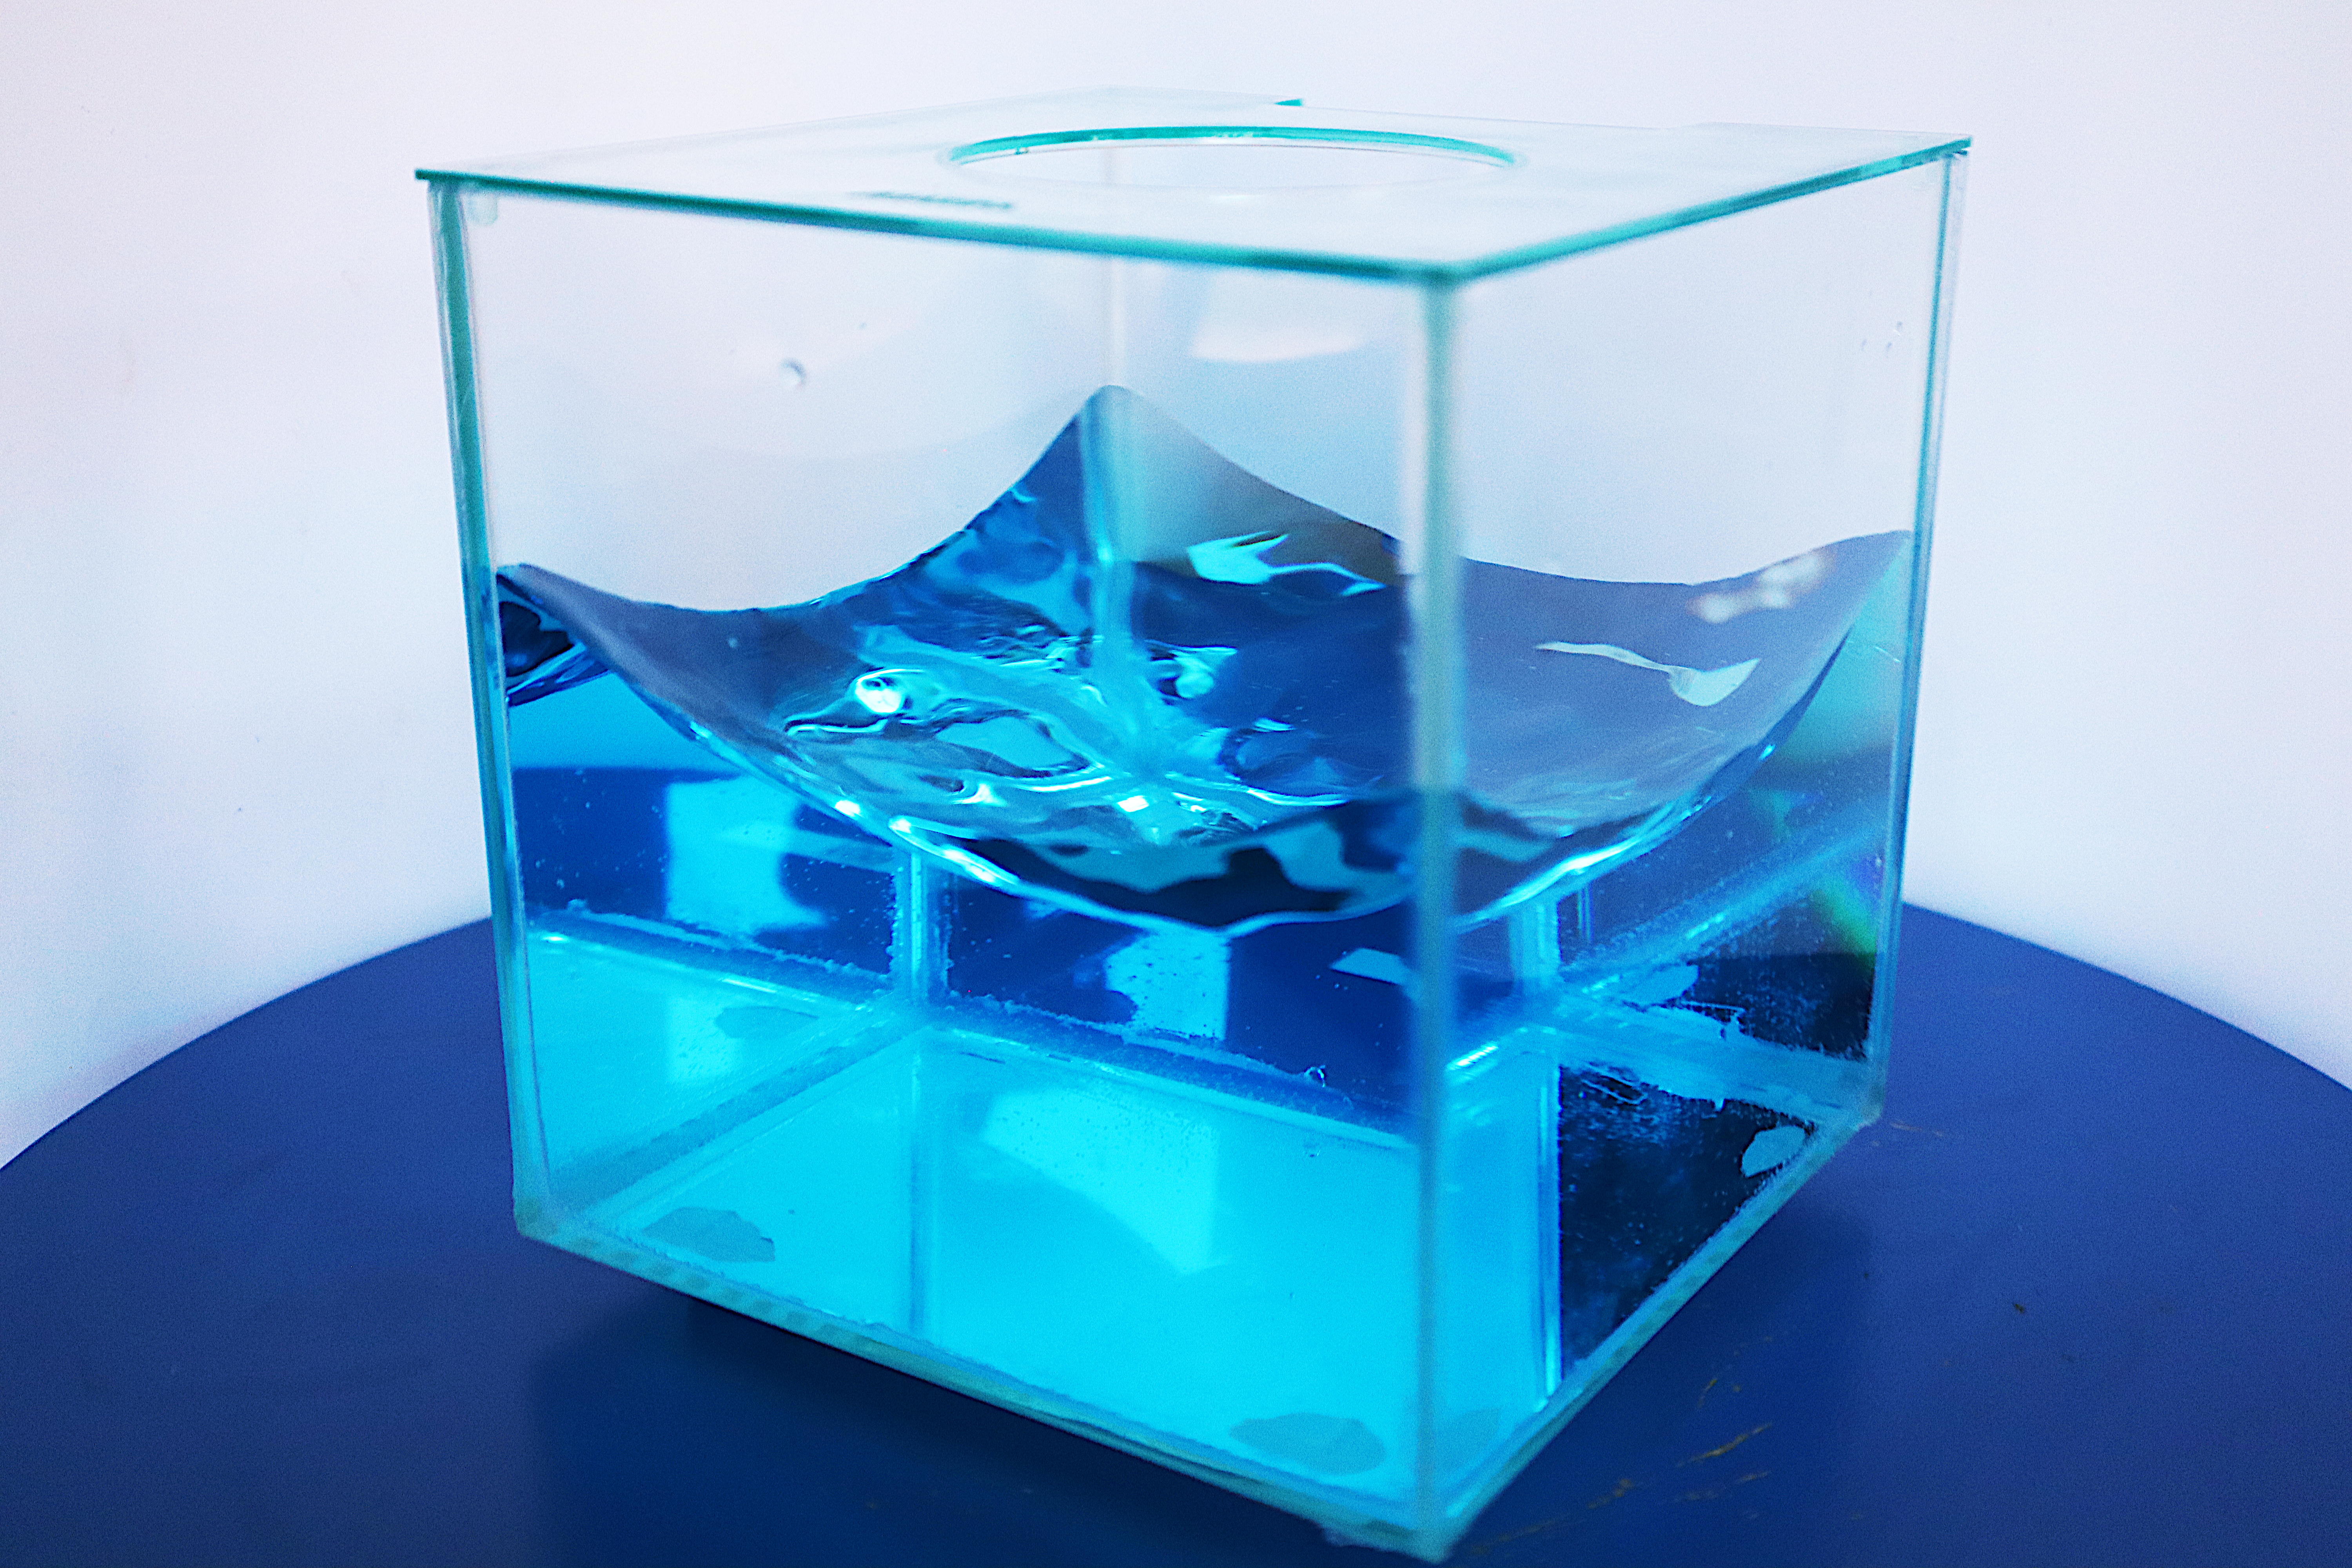
\includegraphics[width=0.7\linewidth]{Figures/Chapter3/fig_water_bucket.jpg}
\caption{A tank of water is smoothly spun up, causing the water to ``climb'' the sides of the tank.}
\label{fig_bucket}
\end{figure}

The $x$ component of Euler's equation, with $\symbfup{g} = [0,0,-g]$, is
\[
\frac{\partial u}{\partial t} + u\frac{\partial u}{\partial x} +  v\frac{\partial u}{\partial y} + w\frac{\partial u}{\partial z} = -\frac{1}{\rho} \frac{\partial p}{\partial x}.
\]
But the flow is \emph{steady}, and $u$ doesn't depend on $x$ or $z$.  Substituting in the fluid velocity in equation (\ref{eq_bucket_vel}), this equation reduces to
\begin{equation}
\label{eq_px}
\frac{\partial p}{\partial x} = \rho \Omega^2 x.
\end{equation}
Similarly, the $v$ and $w$ equations reduce to
\begin{equation}
\label{eq_py}
\frac{\partial p}{\partial y} = \rho \Omega^2 y
\end{equation}
and
\begin{equation}
\label{eq_pz}
\frac{\partial p}{\partial z} = -\rho g.
\end{equation}

We can now integrate to find the pressure $p(x, y, z)$.  From equation (\ref{eq_px}) we get
\[
p = \tfrac{1}{2} \rho \Omega^2 x^2 + f(y, z),
\]
where the function $f(y,z)$ is there since equation (\ref{eq_px}) is a \emph{partial} derivative -- we don't just get a constant of integration, but a possible function of the other two variables.  Integrating equation (\ref{eq_py}) gives
\[
p = \tfrac{1}{2} \rho \Omega^2 y^2 + g(x, z),
\]
and integrating equation (\ref{eq_pz}) gives
\[
p = -\rho g z + h(x, y).
\]
By inspection, it's clear that the pressure must be
\[
p(x, y, z) = \tfrac{1}{2} \rho \Omega^2 (x^2 + y^2) - \rho gz + p_1,
\]
where $p_1$ is a constant -- it's the pressure at the origin where $x=y=z=0$.

That's the pressure everywhere in the water.  To find the shape of the free surface, we'll set $p = p_0$ and solve for the height $z$:
\begin{equation}
z = \frac{\Omega^2}{2g} (x^2 + y^2) + \left( \frac{p_1 - p_0}{\rho g} \right).
\end{equation}
This is a \emph{paraboloid} -- see Figure \ref{fig_bucket_para} -- and it matches the shape in the photograph in Figure \ref{fig_bucket}.

\begin{figure}
\centering\includegraphics[width=0.8\linewidth]{Figures/Chapter3/fig_paraboloid}
\caption{The free surface of the spinning bucket problem is a paraboloid. }
\label{fig_bucket_para}
\end{figure}





\section{The Velocity Potential and Stream Function}

\subsection{The Velocity Potential}

For any irrotational flow, where
\[
\curl \uu = \vec{0},
\]
a scalar function $\varphi$ can be defined such that
\begin{equation}
\label{eq_vel_pot}
\boxed{
\uu = \grad \varphi.
}
\end{equation}
Then, since the curl of a gradient is zero, irrotationality is automatically satisfied. The quantity $\varphi$ is called the \emph{velocity potential}.  In addition, from Stokes' theorem, we also have that
\[
\oint \uu \cdot d\vec{l} = \int (\curl \uu) \cdot d\vec{a} = 0,
\]
so that the line integral of $\vec{u}$ around any closed loop in the fluid is zero.  This suggests we could also write the velocity potential as
\begin{equation}
\label{eq_vel_pot2}
\varphi(\vec{r}) = \int_{\mathcal{O}}^{\vec{r}} \uu \cdot d\symbfup{l},
\end{equation}
where $\mathcal{O}$ is an arbitrary point in the fluid.  Incidentally, sorry for the notation -- I'm using the Greek letter phi for three things:  the gravitational potential $\Phi$, the cylindrical coordinate $\phi$, and now the velocity potential $\varphi$.  I hope it's not too confusing in context.

This might be familiar to you from electrostatics, where the electric field is also irrotational and we can define an electric potential.  There's a subtle point that frequently arises in fluid dynamics, though, so be careful.  As long as the region is \emph{simply connected} -- that is, the fluid has no holes in it -- the path between $\mathcal{O}$ and $\vec{r}$ doesn't matter, and this leads to $\varphi$ being a single-valued function.  However, if the region is \emph{multiply connected} -- it has holes, regions where there is no fluid -- the integral \emph{could} depend on the path and $\varphi$ will be a multivalued function of position.  This can happen is the fluid is surrounding an object, something we'll start to encounter more frequently.  Let's investigate this in more detail with two examples.

\begin{example}[Flow past a stagnation point]
\label{ex_stag_pot}
Recall the flow past a stagnation point (from Examples \ref{ex_stag_point1} to \ref{ex_stag_point2}), given by
\[
\uu = [\alpha x, -\alpha y, 0].
\]
This is irrotational flow (but check to be sure!), and to find the velocity potential, we write
\[
\frac{\partial \varphi}{\partial x} = u = \alpha x \quad \text{and} \quad \frac{\partial \varphi}{\partial y} = v = -\alpha y.
\]
Integrating each term and combining gives
\[
\varphi(x, y) = \tfrac{1}{2} \alpha (x^2 - y^2) + c,
\]
where $c$ is the integration constant.  However, since it's the fluid velocity, not the potential, that is the physically meaningful quantity, we can set the constant $c$ to zero without losing anything -- after all, we'll take a derivative of $\varphi$ to get the velocity, and the constant will end up going anyway.

Note that, in this example, $\varphi$ is a single-valued function of $x$ and $y$.  That means that, for any point in the fluid, $\varphi$ has a single value.  This might not always be the case, as our next example will show.
\end{example}

\begin{example}[Line vortex flow]
\label{ex_pot_vortex}
Next, consider the flow
\[
\uu = \frac{\Gamma}{2\pi s} \, \hat{\phi}.
\]
This is the flow around a line vortex, which we've also seen before.  We have to be a bit more careful for this flow -- it's irrotational (we showed that back in Problem \ref{prob_vortex_vorticity}), but not at the origin where it blows up.  To fix this problem, we'll suppose there's \emph{no} fluid there -- maybe there's a cylinder of radius $a$ there instead, covering up the problem area.  That means the fluid domain is $s \ge a$, but it also means there's now a hole in the fluid domain; it's multiply connected.

The potential is found from equation (\ref{eq_vel_pot}) as usual, but in cylindrical coordinates it looks like
\[
\frac{\partial \varphi}{\partial s} = u_s = 0, \quad \frac{1}{s} \frac{\partial \varphi}{\partial \phi} = u_\phi = \frac{k}{s}, \quad \text{and} \quad \frac{\partial \varphi}{\partial z} = u_z = 0.
\]
Integrating this gives
\begin{equation}
\varphi(\phi) = k \phi.
\end{equation}
But note that this isn't a single-valued function -- $\varphi$ has different values at the same point in space:  $\varphi(0) = 0$, but $\varphi(2\pi) = 2\pi k$, and so on.  We'll see later on that this is connected to circulation within the fluid.

\end{example}

Finally, if the fluid is both irrotational \emph{and} incompressible, it must also satisfy the incompressibility condition,
\[
\symbfup{\nabla} \cdot \uu = 0.
\]
If we rewrite this in terms of the potential, we get
\[
\symbfup{\nabla} \cdot \grad \varphi = 0,
\]
or
\begin{equation}
\boxed{
\nabla^2 \varphi = 0.
}
\end{equation}
This is \emph{Laplace's equation}; any irrotational, incompressible fluid must satisfy it.





\subsection{Flow Past a Cylinder}
\label{sec_cylinder}

Working with the velocity potential rather than the velocity itself is often easier; not only is a scalar function easier to work with than a vector field, but Laplace's equation can be easier to solve than Euler's equation, which also contains the pressure of the fluid as an unknown.  As an example of solving Laplace's equation, we'll find the ideal flow past a cylinder oriented perpendicular to the flow.

We'll start with a few basic assumptions.  First, we'll treat this as two dimensional flow, which means the cylinder is effectively infinitely long.  We'll put the cylinder, which has a radius $a$, along the $z$-axis, and the flow will be uniform in the $x$-direction infinitely far away from the cylinder (see Figure \ref{fig_cyl_setup2}):
\begin{equation}
\label{eq_uniform}
\uu (\infty) = U \, \unit{x},
\end{equation}
where $U$ is the constant speed of the flow far away from the cylinder.

\begin{figure}
\centering\includegraphics[width=0.7\linewidth]{Figures/Chapter3/fig_cyl_setup}
\caption{Fluid flows past the cylinder along the $x$-direction.}
\label{fig_cyl_setup2}
\end{figure}

The other assumption we'll make is that the flow is irrotational.  This seems like a leap to make, though, since we don't even know what the flow \emph{is} yet.  But remember the vorticity equation (equation \ref{eq_vorticity}) -- for a steady two dimensional flow, the vorticity is conserved along streamlines.  Since the vorticity at infinity, where the flow is \emph{uniform}, is definitely zero, and every streamline starts and ends at infinity, it follows that the flow is everywhere irrotational.

Wait, is our flow \emph{steady}?  Yes, as long as we examine the problem from the point of view that the flow has been happening for a while and reached a steady state.  In practice, it doesn't take long for the fluid to do this.

To find the fluid velocity around the cylinder, we'll solve Laplace's equation.  It makes sense to use cylindrical coordinates here, given the symmetry of the boundary.  In cylindrical coordinates, then, Laplace's equation is
\begin{equation}
\label{eq_laplace_cyl}
\ddfdx{\varphi}{s} + \frac{1}{s} \dfdx{\varphi}{s} + \frac{1}{s^2} \ddfdx{\varphi}{\phi} + \ddfdx{\varphi}{z} = 0.
\end{equation}
Of course, we're assuming a two dimensional flow, so the $z$ term we can safely ignore.

Our boundary conditions are straightforward to write down.  First, as $s \to \infty$, we should have the uniform flow given by equation (\ref{eq_uniform}).  But we need the potential rather than the velocity; following similar steps as in the examples above, the potential for uniform flow along the $x$-direction is
\begin{equation}
\label{eq_cyl_bc1}
\varphi = Ux = U s \cos \phi,
\end{equation}
where I've converted the Cartesian coordinates to cylindrical.  Our first boundary condition, then, is that the flow must become this as $s \to \infty$.

Secondly, at $s=a$, we have the actual boundary.  Unlike viscous flows, ideal fluids must ``slip'' along a boundary; in this case, that means we must have the fluid velocity at $s=a$ be purely in the $\unit{\phi}$ direction.  In other words, we need $u_s = 0$; in terms of the potential (using the gradient in cylindrical coordinates), that's
\begin{equation}
\label{eq_cyl_bc2}
\dfdx{\varphi}{s} = 0 \quad \text{at} \quad s=a.
\end{equation}

We'll solve Laplace's equation using separation of variables.  Let
\[
\varphi(s, \phi) = S(s) \Phi(\phi).
\]
Then equation (\ref{eq_laplace_cyl}) becomes
\[
\Phi \frac{d^2S}{ds^2} + \frac{\Phi}{s} \frac{dS}{ds} + \frac{S}{s^2} \frac{d^2 \Phi}{d\phi^2} = 0,
\]
or, dividing by $S\Phi$ and multiplying by $s^2$,
\begin{equation}
\label{eq_cyl_sep}
\frac{s^2}{S} \frac{d^2S}{ds^2} + \frac{s}{S} \frac{dS}{ds} = -\frac{1}{\Phi} \frac{d^2 \Phi}{d \phi^2}.
\end{equation}
The left hand side of the equation is a function of $s$ only, while the right hand side is a function of $\phi$ only; they must therefore both be equal to a constant.  We'll call the this separation constant $k^2$.  The $\phi$ equation is then
\[
\frac{d^2 \Phi}{d\phi^2} = -k^2 \Phi,
\]
which has the solution
\[
\Phi (\phi) = A \sin k\phi + B \cos k\phi.
\]

We can apply our first boundary condition, equation (\ref{eq_cyl_bc1}), right away to eliminate the sine term, since we need only a cosine dependence as $s \to \infty$.  Comparing the form of equation (\ref{eq_cyl_bc1}) with our solution, we furthermore must have $k=1$.  Thus 
\begin{equation}
\Phi(\phi) = B \cos \phi.
\end{equation}

The radial part of equation (\ref{eq_cyl_sep}) (with $k = 1$) now reads
\[
s^2 \frac{d^2S}{ds^2} + s \frac{dS}{ds} - S = 0.
\]
We've seen this differential equation before; it can solved by trying a power-law solution of the form $S(s) = s^m$.  The general solution is
\[
S(s) = Cs + \frac{D}{s}.
\]
But our second boundary condition, equation (\ref{eq_cyl_bc2}), was that the first derivative of the potential goes to zero at $s=a$.  That means
\[
\frac{dS}{ds} = \left. \left( C - \frac{D}{s^2} \right)  \right|_{s=a} = 0,
\]
and so $D = a^2 C$.

Combining the radial and angular equations gives us
\[
\varphi(s, \phi) = S(s) \Phi(\phi) = C \left( s+\frac{a^2}{s} \right) \cos \phi,
\]
where I absorbed the constants into $C$.  One more comparison with our boundary condition, equation (\ref{eq_cyl_bc1}), tells us that $C = U$.  So our solution to Laplace's equation is, finally, 
\begin{equation}
\varphi(s, \phi) = U \left( s+\frac{a^2}{s} \right) \cos \phi.
\end{equation}

That's the potential; what about the fluid velocity?  No problem:
\[
\uu = \grad \phi,
\]
so
\begin{equation}
u_s(s, \phi) = U \left( 1 - \frac{a^2}{s^2} \right) \cos \phi
\end{equation}
and
\begin{equation}
u_\phi(s, \phi) = -U \left( 1 + \frac{a^2}{s^2} \right) \sin \phi.
\end{equation}
From $\uu$, we can sketch streamlines, which are shown in Figure \ref{fig_cyl_streamlines}.

\begin{figure}
\centering\includegraphics[width=0.7\linewidth]{Figures/Chapter3/fig_cylinder_stream}
\caption{The streamlines for the flow around the cylinder.  Note that there are stagnation points upstream and downstream of the cylinder ($\phi = 0$ and $\phi = \pi$), and the fluid has greatest velocity at the top and bottom ($\phi = \pi2$ and $\phi = 3\pi/2$).}
\label{fig_cyl_streamlines}
\end{figure}

Let's examine the flow in a little more detail.  Note that, as necessary, $u_s=0$ at $s=a$.  On the boundary, the flow is purely angular, with speed 
\[
u_\phi = -2U \sin \phi \quad \text{at} \quad s=a.
\]
At $\phi = 0$ and $\phi = \pi$, then $u_\phi = 0$ and there is a stagnation point there (see Figure \ref{fig_cyl_streamlines}).  There is a maximum speed at $\phi = \pi/2$ and $\phi = 3\pi/2$ of
\[
u_{\phi, \text{max}} = 2U \quad \text{at} \quad s=a.
\]

What about the pressure in the fluid?  Well, we could apply Euler's equation to find it, but Bernoulli's principle provides a shortcut.  Since the flow is irrotational, $\grad H = 0$ and $H = p/\rho + \tfrac{1}{2} \uu^2 + gz = $ constant everywhere in the fluid.  In our analysis, though, we'll neglect the gravity term; we're only looking at the $(s, \phi)$ dependence of the pressure here, and gravity will only impose an overall vertical pressure gradient.

Let's first evaluate $H$ at infinity, where $\uu = (U,0,0)$ and we'll label the pressure $p_\infty$.  Then
\[
H = \frac{p_\infty}{\rho} + \tfrac{1}{2} U^2.
\]
Elsewhere in the fluid, it's
\[
H = \frac{p(s, \phi)}{\rho} + \tfrac{1}{2} \uu^2,
\]
where
\[
\uu^2 = \uu \cdot \uu = u_s^2 + u_\phi^2 = U^2 \left( 1 + \frac{a^4}{s^4} - 2\frac{a^2}{s^2} \cos 2\phi \right)
\]
(that last step required some algebra to clean up, though).  Since $H$ is constant, we have
\[
\frac{p(s, \phi)}{\rho} + \tfrac{1}{2} U^2 \left( 1 + \frac{a^4}{s^4} - 2\frac{a^2}{s^2} \cos 2\phi \right) = \frac{p_\infty}{\rho} + \tfrac{1}{2} U^2.
\]
Rearranging gives the pressure,
\begin{equation}
p(s, \phi) = p_\infty + \tfrac{1}{2} \rho \frac{a^2}{s^2} U^2 \left( 2 \cos 2\phi - \frac{a^2}{s^2} \right).
\end{equation}
Figure \ref{fig_cyl_pressure} shows the pressure around the cylinder; there is a region of high pressure at $\phi = 0$ and $\phi = \pi$, with low pressure at $\phi = \pi/2$ and $\phi = 3\pi/2$.  Not surprisingly, this is opposite the fluid velocity -- expected, since Bernoulli's theorem holds here.

\begin{figure}[t]
\centering\includegraphics[width=0.8\linewidth]{Figures/Chapter3/fig_cylinder_pressure}
\caption{The pressure field of fluid flowing past a cylinder.  The dark red regions are areas of high pressure, while the blue areas are low pressure.  The streamlines are shown as well.}
\label{fig_cyl_pressure}
\end{figure}


\subsection{The Stream Function}

Let's take a break from thinking about irrotational flow for a moment, and instead consider flow that is incompressible (it's important to note that the velocity potential $\varphi$ doesn't require incompressibility to describe flow, just irrotationality).  We'll impose the further restriction that it is also two dimensional only -- so $\vec{u} = [u(x, y, t), v(x, y, t), 0]$.  In this case, we'll define the \emph{stream function} $\psi$ by
\begin{equation}
\label{eq_stream_def}
\boxed{
\vec{u} = \curl (\psi \, \unit{z}).
}
\end{equation}

Why this particular function?  Well, consider it in Cartesian coordinates,
\begin{equation}
u = \dfdx{\psi}{y} \quad \text{and} \quad v = - \dfdx{\psi}{x}.
\end{equation}
With this definition, the incompressibility equation is automatically satisfied:
\[
\grad \cdot \uu = \dfdx{u}{x} + \dfdx{v}{y} = \dfdx{}{x} \left( \dfdx{\psi}{y} \right) + \dfdx{}{y} \left( - \dfdx{\psi}{x} \right) = 0,
\]
since the order of the derivatives doesn't matter.  Compare this with the velocity potential:  it ensures irrotational flow, while the stream function ensures incompressible flow, at the cost of requiring it to be two dimensional.  By the way, in cylindrical coordinates, this definition becomes
\begin{equation}
\label{eq_stream_cyl}
u_s = \frac{1}{s} \dfdx{\psi}{\phi} \quad \text{and} \quad u_\phi = - \dfdx{\psi}{s}.
\end{equation}

You might be wondering why the stream function has that particular name -- and it turns out the reason is one of its most useful features.  Note that
\[
(\vec{u} \cdot \grad ) \psi = u\dfdx{\psi}{x} + v\dfdx{\psi}{y} = \dfdx{\psi}{y} \dfdx{\psi}{x} + \left( -\dfdx{\psi}{x} \right) \dfdx{\psi}{y} = 0.
\]
Remember what this means from Section \ref{sec_tot_deriv} -- that $\psi$ is constant on streamlines; hence the name.  If we know the stream function $\psi$, we'll now be able to easily plot the streamlines:  just set $\psi$ to a constant.  Different values of the constant will give you different streamlines.


\begin{example}[Flow past a stagnation point]
\label{ex_stag_psi}
Let's continue on from Example \ref{ex_stag_pot} and find the stream function for the flow
\[
\vec{u} = [\alpha x, -\alpha y, 0],
\]
which is incompressible (feel free to check) and obviously two dimensional.  From $u = \partial \psi / \partial y$ we get
\[
\dfdx{\psi}{y} = \alpha x,
\]
which integrates to 
\[
\psi(x, y) = \alpha x y + f(x),
\]
where $f(x)$ is some possible function of $x$.  From $v = -\partial \psi / \partial x$, we end up with something similar after integrating,
\[
\psi(x, y) = \alpha x y + g(y),
\]
where again $g(y)$ is our integration ``constant.''  Now, comparing the two equations for $\psi$, it's clear that we must have
\begin{equation}
\psi(x, y) = \alpha x y.
\end{equation}

Streamlines for this flow can be found from setting $\psi$ to a constant, which we'll call $k$:
\[
\psi = \alpha x y = k,
\]
or
\[
y = \frac{k}{\alpha x} = \frac{c}{x},
\]
where $c = k/\alpha$.  This exactly matches the equation we found back in Example \ref{ex_stag_stream} for the streamlines of a flow about a stagnation point.
\end{example}



\begin{example}[Line vortex flow]
\label{ex_vortex_psi}
For the line vortex flow, from Example \ref{ex_pot_vortex} with
\[
\uu = \frac{\Gamma}{2\pi s} \, \hat{\phi},
\]
the process to finding the stream function is similar, but we have to use cylindrical coordinates.  From equation (\ref{eq_stream_cyl}), we get
\[
u_s = 0 = \frac{1}{s} \dfdx{\psi}{\phi} \quad \text{and} \quad u_\phi = \frac{\Gamma}{2\pi s} = -\dfdx{\psi}{s}.
\]
From the first equation we just find that $\psi$ has no $\phi$ dependence, and from the second, upon integrating, we get
\[
\psi(s, \phi) = -\frac{\Gamma}{2\pi} \ln s.
\]

Once again we can find the streamlines from the stream function by setting $psi$ to a constant (call it $k$ again).  Doing so and solving for $s$ gives
\[
s = e^{-2\pi k / \Gamma} = \text{constant}.
\]
This makes sense, since we know this is circular flow -- the streamlines are circles of constant radius $s$.
\end{example}

Like the velocity potential, the stream function satisfies Laplace's equation as long as the flow is both incompressible and irrotational -- although here we need the additional constraint of two dimensional flow as well.  The proof is straightforward: start with the condition for irrotational flow, $\curl \uu = \vec{0}$, and substitute in the definition of the stream function from equation (\ref{eq_stream_def}) to get
\[
\curl [ \curl (\psi \, \unit{z}) ] = \vec{0}.
\]
But we can expand the curl of a curl as
\[
\curl [ \curl (\psi \, \unit{z}) ] = \grad [\grad \cdot (\psi \, \unit{z})] - \nabla^2 (\psi \, \unit{z}) = \vec{0},
\]
and, for two dimensional flow, the first term goes to zero, so we're left with
\begin{equation}
\boxed{
\nabla^2 \psi = 0.
}
\end{equation}
So both the velocity potential $\varphi$ and the stream function $\psi$ satisfy Laplace's equation for two dimensional, irrotational, incompressible flow.  Although not every problem in fluid dynamics satisfies these restriction, many do, and we'll exploit this in the next chapter to investigate some interesting and complex situations.




\section*{Problems}
\addcontentsline{toc}{section}{Problems}
\markright{Problems}%

\begin{problem}[Yet more vector calculus]
\label{prob_vc3}
Show that, for any vector field $\symbfup{v}$, you can write
\[
(\symbfup{v} \cdot \grad ) \symbfup{v} = (\curl \symbfup{v}) \times \symbfup{v} + \grad(\tfrac{1}{2} \symbfup{v}^2).
\]
\end{problem}

\begin{problem}[Please, no more vector calculus]
\label{prob_vc4}
Show that, for any two vector fields $\symbfup{F}$ and $\symbfup{G}$, you can write
\[
\curl (\symbfup{F} \times \symbfup{G}) = (\symbfup{G} \cdot \grad) \symbfup{F} - (\symbfup{F} \cdot \grad) \symbfup{G} + \symbfup{F} (\symbfup{\nabla} \cdot \symbfup{G}) - \symbfup{G} (\symbfup{\nabla} \cdot \symbfup{F})
\]
\end{problem}


\begin{problem}[The Rankine Vortex as a Model for Hurricanes]
A Rankine vortex is defined by the flow (in cylindrical coordinates)
\[
\symbfup{u}  = \left\{
 \begin{array}{l l}
    \Omega s \, \hat{\phi} & \quad \text{if $s < a$}\\
   \frac{\Omega a^2}{s} \, \hat{\phi} & \quad \text{if $s>a$,}
  \end{array} \right.
\]
where $\Omega$ and $a$ are constants (related to the wind speed and size of the ``core,'' respectively).  It serves as a useful model for a number of weather and atmospheric conditions, such as hurricanes, mesocyclones, and tornadoes.  

(a) Plot the wind speed as a function of distance, and calculate and plot the vorticity.

(b) To decide whether it is a useful model for hurricanes, I've provided (online) azimuthal wind speed data and vorticity data for Hurricane Katrina, which devastated New Orleans and the surrounding area in 2005.  The wind speed data has the first column as distance $s$ (in km) and the second column as azimuthal wind speed $u_\phi$ (in m/s).  The vorticity data has the first column as distance $s$ (in km) and the second column as vorticity $\omega$ (in $10^{-4}$ s$^{-1}$).

Use the Rankine vortex (RV) to model this hurricane; what values of $\Omega$ and $a$ give you the best fit?  Does the RV model the vorticity with those parameters as well?  Can you make any conclusions about how well the model does (e.g., is it better in some regions versus others?)

(c) Calculate the pressure throughout the hurricane and find the difference in pressure between r = 0 (the eye of the hurricane) and $s \to \infty$ (outside the storm).

(d) Finally, calculate the shape of the free surface (i.e., where the pressure is atmospheric). Plot the surface, and compare this with photos of Katrina -- how does it look?
\end{problem}



\begin{problem}[The force on a cylinder]
\label{prob_force1}
We've already calculated the pressure in the fluid around a cylinder in Section \ref{sec_cylinder}, so it's a short leap to find the total force exerted on the cylinder by the fluid.

Consider Figure \ref{fig_cylinder_force}:  the force (per unit length of the cylinder) on a small angular section of size $a \, d\phi$ is
\[
d\textbf{F} = - p \hat{n}.
\]
Using this, show the total force on the cylinder is zero.  This is called \emph{D'Alembert's paradox} -- there's no drag on the cylinder, despite very obvious physical evidence to the contrary.  Does it make sense that the fluid exerts no force at all on the cylinder as it flows past?  Discuss.

\begin{figure}[t]
\centering\includegraphics[width=0.5\linewidth]{Figures/Chapter3/fig_cyl_force}
\caption{The force on a small angular section of the cylinder.  The force is opposite the normal vector $\hat{n}$.}
\label{fig_cylinder_force}
\end{figure}
\end{problem}


\begin{problem}[Uniform Flow]
\label{prob_uniform_pot}
Consider two dimensional flow that is constant and flows in a direction at an angle $\alpha$ with respect to the $x$ axis (see Figure \ref{fig_uniform_flow_angle}).  

(a) Find the velocity potential $\varphi(x, y)$.

(b) Find the stream function $\psi(x, y)$.

\begin{figure}[t]
\centering\includegraphics[width=0.7\linewidth]{Figures/Chapter3/fig_uniform_flow_angle}
\caption{A constant flow that makes an angle $\alpha$ with the $x$ axis.}
\label{fig_uniform_flow_angle}
\end{figure}
\end{problem}

\begin{problem}[Line source and sink]
\label{prob_line_source}
Consider the two dimensional flow 
\begin{equation}
\uu = \frac{Q}{2\pi s} \, \unit{s},
\end{equation}
where $Q$ is a constant (you might want to compare the form of this flow to the line vortex).  This is called a \emph{line source} if $Q$ is positive and a \emph{line sink} if it's negative.

(a) Produce a vector plot for the flow.

(b) Find the  velocity potential $\varphi(s, \phi)$.

(b) Find the stream function $\psi(s, \phi)$.
\end{problem}

\begin{problem}[Plotting streamlines]
Consider the two dimensional flow
\[
\uu = [2x+3, -2y].
\]

(a) Show that the flow is irrotational and incompressible.

(b) Find the stream function $\psi(x, y)$ and plot the streamlines.
\end{problem}


\chapter{Potential Flow}

%
%  SECTION 4.1 - THE COMPLEX POTENTIAL
%

\section{The Complex Potential}

In the previous chapter, we saw that an irrotational fluid can be described by the \emph{velocity potential} $\varphi$, defined by
\begin{equation}
\vec{u} = \grad \varphi.
\end{equation}
If, instead, the fluid is both two dimensional and incompressible, it can be described by the stream function, $\psi$, defined via
\begin{equation}
\vec{u} = \grad \times (\psi \, \unit{z}).
\end{equation}
Now, if we have a two dimensional fluid that is both irrotational \emph{and} incompressible, then we can use either $\varphi$ \emph{or} $\psi$ to describe it; in Cartesian coordinates, we have
\begin{equation}
\label{eq_u_phi_psi}
u = \dfdx{\varphi}{x} = \dfdx{\psi}{y} \quad \text{and} \quad v = \dfdx{\varphi}{y} = - \dfdx{\psi}{x}.
\end{equation}

For reasons we'll learn as we go, it's very convenient to define a \emph{third} function, the \emph{complex potential} $w(z)$:
\begin{equation}
\label{eq_complex_pot}
\boxed{
w(z) = \varphi + i \psi.
}
\end{equation}
Unlike the velocity potential and the stream function, the complex potential is a function of a \emph{single} variable -- the complex number $z$.   That makes now a good time to review our knowledge of the complex plane. 

% SECTION 4.1.1 - THE COMPLEX PLANE

\subsection{The Complex Plane}

Consider a complex number $z$:
\begin{equation}
z = x + iy.
\end{equation}
We call $x$ the \emph{real part} of the complex number and $y$ the \emph{imaginary part}.  This can be represented on a Cartesian coordinate system as shown in Figure \ref{fig_complex_plane}; the $x$ axis is the real axis and the $y$ axis the imaginary.  This is called the \emph{complex plane}. 

\begin{figure}
\centering\includegraphics[width=0.7\linewidth]{Figures/Chapter4/fig_complex_plane}
\caption{The complex plane showing the complex number $z = x + iy = s \, e^{i\phi}$.}
\label{fig_complex_plane}
\end{figure}

In addition to using Cartesian coordinates, we can also write the complex number $z$ in polar coordinates; it should be clear from the figure that
\[
z = x + iy = s \cos \phi + is \sin \phi.
\]
Using Euler's famous formula,
\[
e^{i \phi} = \cos \phi + i \sin \phi,
\]
this becomes
\begin{equation}
z = s \, e^{i \phi}.
\end{equation}

Some operations, like multiplying complex numbers, are easier in polar coordinates.  Other operations are unique to complex numbers, such as taking the \emph{complex conjugate} of $z$; this means that every imaginary number $i$ becomes the negative $-i$.  The complex conjugate is denoted with a star:
\[
z^* = x - iy = s \, e^{-i\phi}.
\] 
Although we can square a complex number as normal,
\begin{equation}
\label{eq_z_squared}
z^2 = (x + iy)^2 = x^2 - y^2 + 2ixy,
\end{equation}
an operation that often comes up is the ``complex square,''
\begin{equation}
|z|^2 \equiv z^* z = (x-iy)(x+iy) = x^2 + y^2.
\end{equation}
Notice that the complex square will always give a real number.

Sometimes you'll have a complex number in the denominator of a fraction, which makes it difficult to separate the real and imaginary parts of the complex number -- something we'll do pretty frequently.  You can always get rid of the imaginary part in the denominator by multiplying by the complex conjugate:
\[
\frac{1}{x + iy} = \frac{1}{x+iy} \frac{x - iy}{x-iy} = \frac{x - iy}{x^2 + y^2}.
\]

So far, this is all pretty basic stuff, but we need at least one thing from the more advanced theory of complex analysis -- we'll be working with \emph{complex functions} $f(z)$.  Like complex numbers, complex functions can be separated into real and imaginary parts,
\[
f(z) = f(x + iy) = A(x, y) + i B(x, y),
\]
where $A(x, y)$ and $B(x, y)$ are real-valued functions.  Now, a complex function is \emph{analytic} if $A$ and $B$ are differentiable and satisfy the so-called \emph{Cauchy-Riemann conditions,}
\begin{equation}
\label{eq_cauchy_riemann}
\dfdx{A}{x} = \dfdx{B}{y} \quad \text{and} \quad \dfdx{A}{y} = - \dfdx{B}{x}.
\end{equation}
This means that the complex derivative exists, and can be written as\footnote{This is obviously a drastically shortened and simplified look at complex analysis; for more, see e.g., \emph{Mathematical Method for Physicists}, 4th edition, by Arfken and Weber, Chapter 6.}
\begin{equation}
\frac{df}{dz} = \dfdx{A}{x} + i \dfdx{B}{x} = \dfdx{B}{y} - i \dfdx{A}{y}.
\end{equation}

You might have noticed that the Cauchy-Riemann conditions look a lot like equation (\ref{eq_u_phi_psi}) -- the relationship between the velocity potential and the stream function.  This is the connection to fluid dynamics:  by construction, the complex potential $w(z)$ is an analytic complex function, which means we can write the derivative of it as
\begin{equation}
\label{eq_w_deriv}
\boxed{
\frac{dw}{dz} = \dfdx{\varphi}{x} + i \dfdx{\psi}{x} = u - iv.
}
\end{equation}
Thus the derivative of the complex potential is related to the speed of the fluid by
\[
|\vec{u} | = \left| \frac{dw}{dz} \right| = \sqrt{ \left( \frac{dw}{dz} \right)^* \left( \frac{dw}{dz} \right) }.
\]
This gives us a powerful tool to examine some pretty complicated flows.


% SECTION 4.1.2- BASIC FLOWS

\subsection{Basic Flows}

Although we're restricted to two dimensional, incompressible, irrotational flows, the complex potential is nonetheless a useful description of fluid flow in a variety of cases.  We'll start here with four basic flows, and will build up to fluid flow around a wing of an airplane, all the while using tools of complex analysis.

\begin{figure}
\centering\includegraphics[width=0.6\linewidth]{Figures/Chapter4/fig_basic_flows}
\caption{Four basic potential flows.  Upper left: uniform flow at an angle $\alpha$.  Upper right: flow about a stagnation point.  Lower left: a line vortex.  Lower right: a line source.}
\label{fig_basic_flows}
\end{figure}

\begin{example}[Uniform flow]
To start, consider a simple flow that is uniform everywhere.  We'll suppose it flows at an angle $\alpha$ with the $x$ axis, so that the velocity is
\begin{equation}
\vec{u} = [U\cos \alpha, U\sin \alpha, 0].
\end{equation}
Problem \ref{prob_uniform_pot} asked you to work out the details, but the velocity potential in this case is
\begin{equation}
\varphi (x, y) = U(x \cos\alpha + y\sin\alpha)
\end{equation}
and the stream function is
\begin{equation}
\psi (x, y) = U(y \cos\alpha - x\sin\alpha).
\end{equation}

To find the complex potential, we'll start with equation (\ref{eq_complex_pot}) to get
\[
w = \varphi + i\psi = U(x \cos\alpha + y\sin\alpha) + iU(y \cos\alpha - x\sin\alpha).
\]
We can simplify this with a bit of rearranging:
\[
w = U \left[ (x+iy) \cos\alpha - i(x+iy) \sin\alpha \right].
\]
But $z = x+iy$ so we have
\[
w = Uz(\cos\alpha - i\sin\alpha),
\]
or, using Euler's formula,
\begin{equation}
w(z) = Uze^{-i\alpha}.
\end{equation}
This is the complex potential for uniform flow at an angle $\alpha$.  Note that is is a function only of $z$ -- all the $x$s and $y$s have disappeared, which is necessary for the complex potential.
\end{example}

\begin{example}[Stagnation point flow]
Let's return to a flow we've studied plenty already, the flow about a stagnation point,
\[
\vec{u} = [\alpha x, -\alpha y, 0].
\]
In Example \ref{ex_stag_pot} we found that the velocity potential was
\[
\varphi (x, y) = \frac{1}{2} \alpha (x^2 - y^2),
\]
and in Example \ref{ex_stag_psi} we found the stream function,
\[
\psi(x, y) = \alpha xy.
\]

The complex potential for this flow is
\[
\begin{split}
w & = \varphi + i\psi = \frac{1}{2} \alpha (x^2 - y^2) + i\alpha xy \\
& = \frac{1}{2} \alpha ( x^2 - y^2 + 2ixy ).
\end{split}
\]
If this doesn't look familiar, take a look at equation (\ref{eq_z_squared}) -- the term in the brackets is just $z^2$, so the complex potential is
\begin{equation}
w(z) = \frac{1}{2} \alpha z^2.
\end{equation}

\end{example}


\begin{example}[A line vortex]
\label{ex_line_vortex_w}
Another familiar flow is the line vortex, covered in Examples \ref{ex_pot_vortex} and \ref{ex_vortex_psi}.  For reference, the velocity for this flow is
\[
\vec{u} = \frac{\Gamma}{2\pi s} \, \unit{\phi},
\]
and the velocity potential and stream function are
\[
\varphi(s, \phi) = \frac{\Gamma \phi}{2\pi} \quad \text{and} \quad \psi(s, \phi) = -\frac{\Gamma}{2\pi} \ln s.
\]
We'll construct the complex potential in the same way as above, but we'll have to use polar coordinates to build the complex number $z$.  We have
\[
w = \frac{\Gamma \phi}{2\pi}  -i\frac{\Gamma}{2\pi} \ln s
\]
and can pull out a factor of $-i\Gamma / 2 \pi$ to get
\[
w = -\frac{i\Gamma}{2\pi} \left( i\phi + \ln s \right).
\]
Now we'll have to use a bit of a trick:  we can write $i\phi$ as
\[
i\phi = \ln \left( e^{i\phi} \right),
\]
and then combine the two natural logarithms to get
\[
w = -\frac{i\Gamma}{2\pi} \ln \left( s e^{i\phi} \right).
\]
But in polar coordinates, $z = s e^{i\phi}$, so we finally have
\begin{equation}
w(z) = -\frac{i\Gamma}{2\pi} \ln z.
\end{equation}

\end{example}

\begin{example}[A line source]
For our final example, consider the flow about a \emph{line source},
\begin{equation}
\vec{u} = \frac{Q}{2\pi s} \, \unit{s},
\end{equation}
where $Q$ is a constant.  Problem \ref{prob_line_source} has some more information, but the velocity potential is
\begin{equation}
\varphi (s, \phi) = \frac{Q}{2\pi} \ln s,
\end{equation}
while the stream function is
\begin{equation}
\psi(s, \phi) = \frac{Q \phi}{2\pi}.
\end{equation}

The complex potential for this flow is
\begin{equation}
w(z) = \frac{Q}{2\pi} \ln z,
\end{equation}
and you can work out the details yourself in Problem \ref{prob_line_source_w}.
\end{example}

These four basic flows are shown in Figure \ref{fig_basic_flows} and summarized in Table \ref{tab_pot_flows}; we'll be working with them a lot.  However, one of the powerful things about the complex potential is that they can \emph{add together}.  This is possible because, since both $\varphi$ and $\psi$ are solutions to Laplace's equation, so too is the complex potential $w = \varphi + i\psi$.  And since the Laplacian is a linear operator, any combination of solutions is a solution as well.

\begin{table}[t]
\caption{Four basic potential flows.}
\centering
  \begin{tabular}{l|l|l}
  Flow & Velocity & Complex Potential \\ \hline
  Uniform flow & $\vec{u} = [U\cos \alpha, U\sin \alpha]$ &  $w(z) = Uz e^{-i\alpha}$ \\
  Stagnation point & $\vec{u} = [\alpha x, -\alpha y]$ &  $w(z) = \frac{1}{2} \alpha z^2$ \\
  Line vortex & $\vec{u} = \frac{\Gamma}{2\pi s} \unit{\phi}$ & $w(z) = -\frac{i\Gamma}{2\pi} \ln z $ \\
  Line source & $\vec{u} = \frac{Q}{2\pi s} \unit{s}$ & $w(z) = \frac{Q}{2\pi} \ln z$
  \end{tabular}
  
  \label{tab_pot_flows}
\end{table}


For example, suppose we combine a line source with a uniform flow (with angle $\alpha = 0$):
\[
w(z) = Uz + \frac{Q}{2\pi} \ln z.
\]
This complex potential is a perfectly valid description of \emph{some} fluid flow -- it's incompressible and irrotational and satisfies Laplace's equation.  Now, whether or not this is flow that we actually \emph{see} is up to experiment to test; in this case the flow represents fluid around an object called a \emph{Rankine half body}.

We can investigate this flow further by finding the stream function and plotting streamlines.  Remember that $\psi$ is the imaginary part of the complex potential,
\[
\psi = \operatorname{Im}(w).
\]
Finding the imaginary part isn't always simple for a general complex potential, although in this case it's not difficult and you should try it on your own.  I'll discuss this a bit more in the next section; for now, the streamlines are plotted in Figure \ref{fig_uniform_source}.  It's not difficult to imagine how a flow like this might arise -- the red streamline could be the boundary of an object in the fluid, and the flow is passing this object.  This is because for ideal fluids the fluid must ``slip'' along a boundary (there's no no-slip condition for ideal fluids), meaning the boundary must be a streamline.  This boundary condition will play an important role in our next example.

\begin{figure}
\centering\includegraphics[width=0.7\linewidth]{Figures/Chapter4/fig_uniform_source}
\caption{Streamlines for a flow that includes both uniform flow and a line source.}
\label{fig_uniform_source}
\end{figure}


% SECTION 4.1.3 - METHOD OF IMAGES

\subsection{Method of Images}
\label{sec_images}

Consider a single line vortex, but we'll modify the flow in two ways:  first, by moving it to a new position $z_0 = d$ along the $x$ axis, and secondly by putting a wall at $x=0$, effectively having the fluid in the domain $x>0$ only.  This is shown in Figure \ref{fig_mirror_wall}.  Now, the first adjustment is easy to make, since moving the line vortex location just means shifting the origin in the opposite direction; in general, a line vortex at a location $z_0 = x_0 + iy_0$ in the complex plane is given by
\begin{equation}
\label{eq_line_vortex_z0}
w(z) = -\frac{i\Gamma}{2\pi} \ln (z-z_0).
\end{equation}

\begin{figure}
\centering\includegraphics[width=0.75\linewidth]{Figures/Chapter4/fig_mirror_wall}
\caption{A line vortex a distance $d$ from a wall.}
\label{fig_mirror_wall}
\end{figure}

What about the wall?  That's a little trickier, since it's apparent that the flow given in equation (\ref{eq_line_vortex_z0}) doesn't satisfy the boundary conditions -- we need the flow to slip along the wall.  That means we require our flow at $x=0$ to be along the $y$ direction only, so that
\[
u(0, y) = 0.
\]
As shown in Figure  \ref{fig_mirror_wall}, the flow is tangent to the streamlines, and doesn't point just along $y$ at the wall.  In fact, it looks like the fluid is either flowing \emph{into} the wall or \emph{out of} the wall, which doesn't make much sense physically.  How can we adjust our complex potential to satisfy the boundary condition?

Well, never mind for a moment.  Instead, consider a completely \emph{different} problem:  two vortexes, one at $z = d$ as above, and one at $z = -d$; there's no wall in this problem.  The second vortex will have the same strength as the first, but will go in the opposite direction:  $\Gamma_2 = - \Gamma_1$; see Figure \ref{fig_mirror_image}.  Since complex potentials add together, it's simple to write down $w(z)$ for this new flow:
\[
w(z) = -\frac{i\Gamma}{2\pi} \ln (z-d) + \frac{i\Gamma}{2\pi} \ln (z+d)
\]
(notice the plus sign -- the second term is for the vortex that rotates in the opposite sense as the first).  We can simplify this a bit using log rules to get
\begin{equation}
\label{eq_mirror_vortex}
w(z) = -\frac{i\Gamma}{2\pi} \ln \left( \frac{z - d}{z+d} \right).
\end{equation}

Now, \emph{this} flow \emph{does} satisfy the boundary condition -- the two flows from each vortex combine at the wall and the $x$ components of the velocity end up cancelling, giving components along the $y$ direction only.  In other words, this flow slips along the boundary; you can prove this mathematically if you want by trying Problem \ref{prob_mirror_bc}.

\begin{figure}
\centering\includegraphics[width=\linewidth]{Figures/Chapter4/fig_mirror_image}
\caption{Two line vortexes combine to create a flow that slips along the wall.}
\label{fig_mirror_image}
\end{figure}

By adding a second vortex, we've satisfied the boundary conditions of the original problem; this is a technique called method of images, which you might know from electrostatics.  Of course, in the original problem, we had only \emph{one} vortex, not two -- but that's okay, since our second vortex is covered up by the wall.  It's not really there, and our solution is only good for the domain $x>0$.  

Method of images works because our fluid satisfies Laplace's equation, and solutions to Laplace's equation are \emph{unique}: if a complex potential is a solution to Laplace's equation \emph{and} satisfies the boundary conditions of the problem, then it's \emph{the} solution.\footnote{Griffiths has an excellent discussion of uniqueness theorems and Laplace's equation in \emph{Introduction to Electrodynamics}, 4th edition, Chapter 3; as usual there's much more to say about the matter.}

One more thing before we move on.  What does the flow in $x>0$ actually look like?  Figure \ref{fig_mirror_image} gives streamlines for each vortex superimposed, not combined properly.  To find the streamlines, we need the stream function,
\[
\psi = \operatorname{Im}(w).
\]
As I mentioned above, it's not always easy to find the imaginary part of the complex potential, particularly when logarithms are involved.  I'll walk you through a general method for doing so, and we'll start with the polar form of the complex number $z$:
\[
z = s e^{i\phi}.
\]
Here, $s$ is often called the \emph{modulus}, and is the complex absolute value of $z$,
\[
s = |z| = \sqrt{z^*z},
\]
and $\phi$ is called the argument.  Now, if we just have the logarithm of a complex number, that's easy enough to split into real and imaginary parts, and we've already seen the reverse of it in Example \ref{ex_line_vortex_w}:
\[
\ln z = \ln s + i\phi.
\]
Note that the real part of $\ln z$ is the logarithm of the modulus $s$ and the imaginary part is the argument $\phi$.  Careful, though -- in fact, I could add a multiple of $2\pi$ to $\phi$ and still get the same $\ln z$, so there's actually an infinite number of possibilities for the imaginary part of $\ln z$.  Writing it as I did means $\ln z$ is called the \emph{principle value.} This is something we won't have to worry about much, but I wanted to mention it for completeness. 

If we have something more complicated, say the logarithm of a complex function $f(z)$, the idea is the same,
\[
\ln \left[ f(z) \right] = \ln \left| f(z) \right| + i \operatorname{Arg} \left[ f(z) \right].
\]

Now, it might not be simple to find the argument of the function $f(z)$ -- you'll have to split it into its real and imaginary parts, 
\[
f(z) = A(x, y) + iB(x, y),
\]
and then find the argument from
\[
\operatorname{Arg}\left[ f(z) \right] = \operatorname{Arg}\left[ A(x, y) + iB(x, y) \right] = \tan^{-1} \left[ \frac{B(x,y)}{A(x,y)} \right].
\]
Things can once again get complicated in dealing with the arctan function, but luckily we won't have to worry about this much either.  The modulus at least is normally not a problem, since
\begin{equation}
\left| f(z) \right| = \sqrt{ f^*(z) f(z) }.
\end{equation}

In the case of the vortex beside the wall, we can now write
\[
w(z) = -\frac{i\Gamma}{2\pi} \ln \left( \frac{z - d}{z+d} \right) = -\frac{i\Gamma}{2\pi} \left[ \ln \left| \frac{z-d}{z+d} \right| + i \operatorname{Arg} \left( \frac{z-d}{z+d} \right) \right]
\]
or
\[
w(z) = \frac{\Gamma}{2\pi}\operatorname{Arg} \left( \frac{z-d}{z+d} \right) - i \frac{\Gamma}{2\pi} \ln \left| \frac{z - d}{z+d} \right|,
\]
and we can identify the stream function as the imaginary part,
\begin{equation}
\psi(x, y) = \frac{\Gamma}{2\pi} \ln \left| \frac{z - d}{z+d} \right|.
\end{equation}
Careful, though -- there are still complex numbers $z$ in that equation for $\psi$, which should be a real function.  However, because the complex absolute value is there, it's guaranteed to be real -- if you work it out (it's a bit of algebra but not too hard), you get
\begin{equation}
\psi(x, y) = -\frac{\Gamma}{2\pi} \ln \sqrt{ \frac{x^2 + y^2 - 2xd + d^2}{x^2 + y^2 + 2xd + d^2} }.
\end{equation}
From the stream function you can plot the streamlines of the flow as shown in Figure \ref{fig_vortex_wall}; notice that one streamline lies directly along the wall.

\begin{figure}
\centering\includegraphics[width=0.9\linewidth]{Figures/Chapter4/fig_vortex_wall}
\caption{The streamlines for a line vortex a distance $d$ from a wall.  The left side shows both vortexes, while the right side shows just the real vortex beside the wall.}
\label{fig_vortex_wall}
\end{figure}


% SECTION 4.1.4 - THE CIRCLE THEOREM

\subsection{The Circle Theorem}

Take a close look at Figure \ref{fig_vortex_wall} -- although the circular streamlines are no longer \emph{concentric}, they are still circular.  That suggests that this complex potential can also work for a line vortex within a \emph{circular} boundary (say, a cylindrical bucket filled with fluid) -- as long as the boundary matches one of the streamlines, our boundary condition will be satisfied and the fluid will slip along the circular wall.

Consider the situation shown in Figure \ref{fig_circular_boundary}.  We'll put the origin of our coordinate system at the centre of the cylindrical bucket (of radius $a$) and orient the $x$ axis so that the line vortex of strength $\Gamma$ is located on it at $x = c_1$.  To ensure a streamline matches the boundary of the cylinder, we'll need a mirror image of the vortex (with opposite circulation $-\Gamma$) on the $x$ axis -- outside the cylinder.  The question is \emph{where} do we put it?

\begin{figure}
\centering\includegraphics[width=0.75\linewidth]{Figures/Chapter4/fig_circular_boundary}
\caption{A line vortex in a circular bucket can be modelled with a mirror image outside the bucket.}
\label{fig_circular_boundary}
\end{figure}

Take a look at the circles on the left side of Figure \ref{fig_vortex_wall} again -- they're a well-known system called \emph{coaxal circles}.  The members of a coaxal system are described by the equation
\begin{equation}
\label{eq_coaxal_circles}
x^2 + y^2 + 2\lambda x + k = 0,
\end{equation}
with different values of $\lambda$ giving different circles.  These two sets of circles have \emph{limiting points} at $x = \pm \sqrt{k}$ -- that's where they converge to a circle of radius zero.  In our problem here, the positions of the two line vortexes at $x=c_1$ and $x=c_2$ would be the limiting points. From equation (\ref{eq_coaxal_circles}) you can derive a relationship between the radius $a$ of one of the circles and the two limiting points; it turns out to be
\[
a^2 = c_1 c_2.
\]
If we have a vortex at $x=c_1$ inside the cylinder, placing a mirror vortex at 
\begin{equation}
c_2 = \frac{a^2}{c_1}
\end{equation}
will give streamlines that match the boundary.  The complex potential of a vortex in a cylindrical bucket a distance $c$ from the centre is therefore
\begin{equation}
w(z) = -\frac{i\Gamma}{2\pi} \ln (z-c) + \frac{i\Gamma}{2\pi} \ln (z-a^2/c)
\end{equation}
(I've dropped the subscript ``1'' from $c$ since we don't need $c_2$ anymore), and the streamlines are shown in Figure \ref{fig_vortex_cylinder}.

%\begin{figure}
%\centering\includegraphics[width=0.75\linewidth]{Figures/Chapter4/fig_circular_inset}
%\caption{The streamlines of the two vortexes combine to give a streamlines that exactly matches the cylinder.}
%\label{fig_circular_inset}
%\end{figure}

\begin{figure}
\centering\includegraphics[width=0.5\linewidth]{Figures/Chapter4/fig_vortex_cylinder}
\caption{The streamlines of a line vortex within a circular cylinder.}
\label{fig_vortex_cylinder}
\end{figure}

The idea of placing a vortex in a flow to get a circular streamline is very general -- and powerful.  The Milne-Thompson Circle Theorem gives us a way to add a circular streamline to any irrotational, incompressible flow, and is given by the following:
\begin{theorem}[Milne-Thompson Circle Theorem]
Consider a flow described by the complex potential
\[
w = f(z),
\]
and any singularities of $f(z)$ (in other words, where it goes to infinity) occur in the region $|z| > a$.  Then the new complex potential
\begin{equation}
w = f(z) + f^*(a^2 / z^*)
\end{equation}
describes a flow that has the same singularities as $f(z)$ in $|z| > a$ \emph{and} has the circle $|z| = a$ as a streamline.
\end{theorem}

This is straightforward to prove.  The circle $|z| = a$ can be written as
\[
|z|^2 = z^* z = a^2,
\]
or
\[
z^* = \frac{a^2}{z}.
\]
That means that, on the circle itself,
\[
w = f(z) + f^*(a^2/z^*) = f(z) + f^*(z).
\]
But the function $f(z) + f^*(z)$ is a \emph{real} function; suppose we write $f(z) = A(x, y) + iB(x, y)$, in which case it's easy to see that 
\[
f(z) + f^*(z) = A(x, y) + iB(x,y) + A(x, y) - iB(x, y) = 2A(x, y),
\]
and the imaginary part has cancelled. If $w(z)$ is a \emph{real} function on the circle, then it's imaginary component must be zero:
\[
\psi(x, y) = \operatorname{Im}(w) = 0.
\]
Never mind the zero -- the important thing is to see that $\psi$ is \emph{constant} along the circle.  That means the circle is a streamline!

What about the singularity part?  Well, any point that is originally outside the circle in $f(z)$ actually ends up \emph{inside} the circle in $f^*(a^2/z^*)$, so no new singularities outside $|z| = a$ are created -- that means the new flow has the same singularities as the original flow.

%
% SECTION 4.2 - FLOW PAST OBJECTS
%

\section{Flow Past Objects}



% SECTION 4.2.1 - FLOW PAST A CYLINDER

\subsection{Flow Past a Cylinder}

As a simple example of the Circle Theorem, consider starting with uniform flow with angle $\alpha = 0$, given by
\[
w(z) = Uz.
\]
Using the Circle Theorem we get
\[
w(z) = Uz + \left[ U \frac{a^2}{z^*} \right]^*
\]
or
\begin{equation}
w(z) = U \left( z + \frac{a^2}{z} \right).
\end{equation}
This is the complex potential for a flow that is uniform at infinity but has a circular streamline centred at the origin with radius $a$; see Figure \ref{fig_uniform_circle}. The streamlines outside the circular streamline might look familiar if you recall Section \ref{sec_cylinder}, and we'll examine them closely in a moment.  But what about the streamlines interior to the circle?  They're similar to the streamlines for a \emph{doublet} flow, in which $w \propto z^{-1}$, but that doesn't really matter -- in fact, if we ``cover up'' the fluid interior to $|z| = a$ with, say, a circular cylinder, then what we've done is find the complex potential for flow around that cylinder.

\begin{figure}
\centering\includegraphics[width=0.7\linewidth]{Figures/Chapter4/fig_uniform_circle}
\caption{The streamlines for the flow generated by applying the Circle Theorem to a uniform flow.}
\label{fig_uniform_circle}
\end{figure}

Does our solution match the one we found earlier in Section \ref{sec_cylinder}?  We can find the velocity potential and stream function easily enough (see Problem \ref{prob_circlular_cylinder}); they are
\begin{equation}
\varphi(s, \phi) = U \left( s + \frac{a^2}{s} \right) \cos\phi
\end{equation}
and
\begin{equation}
\psi(s, \phi) = U \left( s - \frac{a^2}{s} \right) \sin\phi.
\end{equation}
We can also find the velocity of the flow, either from the potential or stream function, or from the derivative of the complex potential directly using equation (\ref{eq_w_deriv}); either way, we get
\begin{equation}
u_s(s, \phi) = U \left( 1 - \frac{a^2}{s^2} \right) \cos\phi
\end{equation}
and
\begin{equation}
u_\phi(s, \phi) = U \left( 1 + \frac{a^2}{s^2} \right) \sin\phi.
\end{equation}
These do indeed match the flow we found earlier -- by much more laborious means (solving Laplace's equation).  It's hard to overstate just how powerful the Circle Theorem can be; we found in a few lines what took us four pages of solving a partial differential equation before.

But we can do more in this case.  It's trivial to add an angle $\alpha$ to the uniform flow, for example; in that case we start with the complex potential
\[
w(z) = Uz e^{-i\alpha}
\]
and get, using the Circle Theorem,
\begin{equation}
w(z) = U \left( ze^{-i\alpha} + \frac{a^2}{z}e^{i\alpha} \right).
\end{equation}
We could also add a line vortex, placed at the origin, to our flow.  This wouldn't change the fact that there's a circular streamline at $|z| = a$, since the line vortex has circular streamlines, but would change the flow $u_\phi$ at the surface of the cylinder -- in effect, we're adding \emph{circulation} to the flow, as we'll see.  Remember, complex potentials add together, so the flow with a line vortex is simply
\begin{equation}
\label{eq_uniform_circle}
w(z) = U \left( ze^{-i\alpha} + \frac{a^2}{z}e^{i\alpha} \right) - \frac{i\Gamma}{2\pi} \ln z.
\end{equation}

\begin{figure}
\centering\includegraphics[width=0.75\linewidth]{Figures/Chapter4/fig_cylinder_circ}
\caption{Streamlines for flow around a circular cylinder at an angle $\alpha = \pi/6$.  Upper left: circulation $\Gamma = 0$.  Upper right: circulation $\Gamma = -2\pi Ua$.  Lower left: circulation $\Gamma = -4\pi Ua$.  Lower right: circulation $\Gamma = -6\pi Ua$.}
\label{fig_cylinder_circ}
\end{figure}

Streamlines with circulation in the flow are shown in Figure \ref{fig_cylinder_circ}.  Something interesting happens as the circulation $\Gamma$ increases:  notice that the two stagnation points, normally at opposite ends of the cylinder, come closer together as the circulation increases, until 
\[
\Gamma = \pm 4\pi U a,
\]
when they combine to form just one stagnation point.  If the circulation is greater than this, they disappear completely -- we now have fluid circulating completely around the cylinder, as you can see by the streamlines in the lower right part of Figure \ref{fig_cylinder_circ} (note that the circulation is negative in the Figure, so that the fluid circulates clockwise around the cylinder; we'll see why I chose this shortly).  You can explore this flow more in Problem \ref{prob_circlular_cylinder}.

Back in Problem \ref{prob_force1} you may have calculated the force of the fluid on a circular cylinder for flow without circulation -- it turned out to be zero, a somewhat surprising result called d'Alembert's paradox.  Because we're dealing with ideal fluids and the flow is symmetric, the fluid is unable to push on the cylinder.  However, this result changes when circulation is added to the flow.  Problem \ref{prob_force2} can walk you through the details of the calculation, but nothing changes for the $x$ component of force -- the fluid still doesn't push on the cylinder in the direction of the oncoming flow -- but there \emph{is} a force in the $y$ direction, perpendicular to the uniform flow:
\begin{equation}
\label{eq_force1}
F_y = -\rho U \Gamma.
\end{equation}
This force is due entirely to the circulation around the cylinder, and if $\Gamma$ is negative, as the examples in Figure \ref{fig_cylinder_circ} show, then the force is upward:  the fluid provides \emph{lift} on the cylinder.  Of course, the wings of an airplane aren't at all circular in cross section, but this essential idea -- that circulation around the object is necessary for lift -- will return when we discuss proper aerofoils.



% SECTION 4.2.2 - CONFORMAL MAPPING

\subsection{Conformal Mapping}

Suppose we have some general complex potential $w(z) = \varphi + i\psi$.  Our goal is to create a \emph{mapping} or \emph{transformation} between the complex plane $z = x+iy$ and a second complex plane, which I'll write with capital letters: $Z = X + iY$.  We'll perform this transformation with the function $f(z)$ such that
\begin{equation}
Z = f(z).
\end{equation}
We'll assume $f(z)$ is an \emph{analytic} complex function, meaning it's differentiable, and that it has an inverse given by
\begin{equation}
z = F(Z)
\end{equation}
(and $F(Z)$ is also an analytic function).

The complex potential is transformed as well -- in the $Z$ complex plane it takes on the form
\begin{equation}
W(Z) = w[F(Z)].
\end{equation}
Now, we can split $W(Z)$ into it's real and imaginary parts,
\begin{equation}
W(Z) = \Phi(X, Y) + i\Psi(X, Y).
\end{equation}
Here's the amazing thing:  because $W$ will be an analytic function of $Z$, $\Phi$ and $\Psi$ will satisfy the Cauchy-Riemann conditions (equation \ref{eq_cauchy_riemann}), and therefore
\begin{equation}
\U(X, Y) = \dfdx{\Phi}{X} = \dfdx{\Psi}{Y} \quad \text{and} \quad \V(X, Y) = \dfdx{\Phi}{Y} = -\dfdx{\Psi}{X}
\end{equation}
represent a possible fluid flow -- that is, the velocity  $\U \, \unit{X} +  \V \, \unit{Y}$ is an irrotational, incompressible flow that satisfies Laplace's equation.

This might seem like a lot to take in at first, but our goal is to use a transformation to map our flow around a circular cylinder to other possible shapes -- including, eventually, a realistic wing shape.  Before we get there, though, let's take a look at a simple example.



\begin{example}[A Simple Conformal Map]
\label{ex_conformal_map}
Consider the map
\[
Z = f(z) = \frac{z^2}{5} + 2,
\]
which has the inverse 
\[
z = F(Z) = \sqrt{5(Z-2)}.
\]
We'll start with the complex potential for uniform flow, $w(z) = Uz$; the left side of Figure \ref{fig_conformal_map} shows the streamlines (blue) as well as lines of constant velocity potential (red).  For uniform flow, these lines are straight and meet at right angles.

Under the map, the complex potential in the $Z$ complex plane becomes
\[
W(Z) = w[F(Z)] = U\sqrt{5(Z-2)};
\]
streamlines for this transformed complex potential are shown on the right panel of Figure \ref{fig_conformal_map}.  The original streamlines are mapped to new streamlines (and similarly for the lines of constant $\varphi$), and are no longer straight -- but notice that they do still cross at right angles.  This is why the mapping is called conformal -- the transformation preserves local angles.

Suppose we look at just one point in the $z$ complex plane, say
\[
z_0 = 1 + i.
\]
The complex potential at that point is $w(z_0) = U(1+i)$.  In the $Z$ complex plane, $z_0$ is mapped to
\[
Z_0 = \frac{2i}{5} + 2,
\]
but the complex potential $W(Z_0)$ has the same value as $w(z_0)$:
\[
W(Z_0) = U\sqrt{5(2i/5 + 2 - 2)} = U\sqrt{2i} = U(1+i).
\]

\end{example}

\begin{figure}
\centering\includegraphics[width=0.75\linewidth]{Figures/Chapter4/fig_conformal_map}
\caption{The effect of the conformal map $f(z) = z^2/5 + 2$ on uniform flow.  The blue lines are the streamlines $\psi = $ constant and the red lines are lines of constant velocity potential $\varphi$.  Left: the original uniform flow, $w(z) = Uz$, in the $z$ complex plane.  Right: the flow under the conformal map $W(Z)$ in the $Z$ complex plane.}
\label{fig_conformal_map}
\end{figure}


When choosing a particular map, there are two things to be careful about.  First, consider the derivative of $W(Z)$.  Writing it as $W(Z) = w(z)$ where $z = F(Z)$, we can use the chain rule to get
\[
\frac{dW}{dZ} = \frac{dw}{dz}\frac{dz}{dZ}.
\]
But recall that $dw/dz = u - iv$, so this says
\begin{equation}
\label{eq_UV}
\U - i\V = \frac{u - iv}{dZ/dz} = \frac{u - iv}{f'(z)},
\end{equation}
using $Z = f(z)$.  If we want the streamlines in the new $Z$ complex plane to match the original streamlines in the $z$ plane at infinity -- far away from the object the fluid is flowing past -- then we'll need
\begin{equation}
f'(z) \to 1 \quad \text{as} \quad |Z| \to \infty.
\end{equation}

The second thing is about the conformal nature of the map.  Normally, local angles are preserved, as we saw in Example \ref{ex_conformal_map}.  However, this is only true if the mapping function $f(z)$ has a non-vanishing first derivative everywhere.  At points where the first derivative is zero, though, the angle changes; in general, the local angle is multiplied by $n$, where $n$ is the order of the first non-vanishing derivative of $f(z)$.  


% SECTION 4.2.4 - FLOW PAST AN ELLIPTICAL CYLINDER

\subsection{Flow Past an Elliptical Cylinder}

Let's try the following transformation:
\begin{equation}
Z = f(z) = z + \frac{c^2}{z},
\end{equation}
where $c$ is a constant.  This is called the \emph{Joukowski transformation}, and was important in the development of the theory of aerodynamics.  Note that the derivative is
\[
f'(z) = 1 - \frac{c^2}{z^2},
\]
so $f'(z) \to 1$ as $|z| \to \infty$; this mapping won't affect the flow far away from the object.  Also note that the first derivative is non-zero almost everywhere, so local angles will be preserved.  However, something interesting happens at $z = \pm c$ -- at that point the first derivative becomes zero, and the first non-vanishing derivative is the \emph{second}.  This means at those points local angles will be \emph{doubled}.

We'll need the inverse of the Joukowski transformation as well; it is given by
\begin{equation}
\label{eq_inverse_jt}
z = \frac{1}{2}Z \pm \sqrt{\frac{1}{4} Z^2 - c^2}.
\end{equation}
Note that, except at the points $Z = \pm 2c$, this inverse is \emph{multivalued}.  In the language of complex analysis, we would say that $Z = \pm 2c$ are \emph{branch points}, and we could cut the plane between them to ensure the inverse is single-valued.  However, in practice, we'll only need the positive root; it turns out that the negative root maps points in the $Z$ complex plane to points within a circle of radius $c$ on the $z$ complex plane, while the positive root maps them to points outside that circle.  Since we're studying fluid flow around objects, there won't be any fluid within that radius anyway -- the object itself will be there.

\begin{figure}
\centering\includegraphics[width=0.75\linewidth]{Figures/Chapter4/fig_jt_ellipse}
\caption{The Joukowski transformation takes a circle in the $z$ complex place to an ellipse in the $Z$ complex plane.  Here the parameter $c = 0.7$.}
\label{fig_jt_ellipse}
\end{figure}

What does the Joulowski transform actually do?  Consider its affect on a circle of radius $a$ in the complex $z$ plane, which is given by
\[
z = a e^{i\phi}.
\]
Applying the transformation leads to 
\[
Z = z + \frac{c^2}{z} = ae^{i\phi} + \frac{c^2}{a} e^{-i\phi}.
\]
This might not look familiar, but with a bit of work we can see what it describes.  Write $Z = X + iY$ and $e^{i\phi} = \cos\phi + i\sin\phi$ and separate $Z$ into its real and imaginary components:
\[
X + iY = \left( a + \frac{c^2}{a} \right) \cos \phi + i \left( a - \frac{c^2}{a} \right) \sin \phi.
\]
Now take the complex conjugate of both sides and rearrange to get
\begin{equation}
\label{eq_ellipse}
\frac{X^2}{(a + c^2/a)^2} + \frac{Y^2}{(a - c^2/a)^2} = 1.
\end{equation}
This is the equation of an ellipse with semimajor axis $a + c^2/a$ and semiminor axis $a - c^2/a$. The shape of the ellipse is controlled by the parameter $c$, so that as $c \to a$, the ellipse gets flatter and flatter.  Figure \ref{fig_jt_ellipse} shows this Joukowski transformation.

To see what the flow around the ellipse looks like, we start with the flow around a circular cylinder of radius $a$ -- including the angle and circulation, as given by equation (\ref{eq_uniform_circle}) -- and use the inverse Joukowski transformation (equation \ref{eq_inverse_jt}) to replace all the $z$s with $Z$s. After a bit of rearranging, the complex potential around an elliptical cylinder is given by
\begin{multline}
\label{eq_ellipse_w}
W(Z) = Ue^{-i\alpha} \left( \frac{1}{2} Z + \sqrt{\frac{1}{4} Z^2 - c^2} \right) + Ue^{i\alpha} \frac{a^2}{c^2} \left( \frac{1}{2} Z - \sqrt{\frac{1}{4} Z^2 - c^2} \right) - \\ \frac{i\Gamma}{2\pi} \ln \left( \frac{1}{2} Z + \sqrt{\frac{1}{4} Z^2 - c^2} \right)
\end{multline}
To find the streamlines we have to extract the imaginary part of this very complicated complex potential.  Although possible, I'll leave it as an exercise for you to try; the streamlines themselves are shown in Figure \ref{fig_ellipse}. Luckily, producing the streamline plot with a computer is much easier than finding the streamlines by hand.

\begin{figure}
\centering\includegraphics[width=0.7\linewidth]{Figures/Chapter4/fig_ellipse}
\caption{The streamlines for flow around an elliptical cylinder, with $c=0.7$, $\alpha = \pi/6$, and $\Gamma= 0$.}
\label{fig_ellipse}
\end{figure}


% SECTION 4.2.5 - FLOW PAST A FLAT PLATE

\subsection{Flow Past a Flat Plate}

The shape of the ellipse is dependent on the parameter $c$ in the Joukowski transformation, and if we let $c \to a$, so that the transformation is
\begin{equation}
Z = z + \frac{a^2}{z},
\end{equation}
the ellipse collapses to a flat plate.  Looking at equation (\ref{eq_ellipse}), we see that the semiminor axis goes to zero, while the semimajor axis becomes $2a$ -- so the plate has a total length of $4a$.  The flow in this case is shown in the left panel of Figure \ref{fig_flat_plate}.

Although it's difficult to see in that streamline plot, there are two points in the flow where the velocity goes to infinity -- there are two \emph{singularities}.  They occur at each edge of the plate, at $Z = \pm 2a$.  To investigate the velocity of the flow, we have to find the derivative $dW/dZ$, which can be lengthy and complicated.  To simplify things for a bit, suppose $\Gamma = 0$; letting $a=c$ in equation (\ref{eq_ellipse_w}) and taking the derivative, we get (with some simplification)
\[
\U - i\V = \frac{dW}{dZ} = U\cos \alpha - i \frac{U \sin \alpha \, Z}{\sqrt{Z^2 - 4a^2}}.
\]
You can see in the imaginary term that the denominator goes to zero as $Z \to \pm 2a$ -- so the $Y$ component of the velocity blows up there and we have a singularity in the flow.

\begin{figure}
\centering\includegraphics[width=\linewidth]{Figures/Chapter4/fig_flat_plate}
\caption{The streamlines for flow around a flat plate with angle $\alpha = \pi/6$.  Left: $\Gamma = 0$.  Right: $\Gamma= -4\pi Ua \sin\alpha$.}
\label{fig_flat_plate}
\end{figure}

Now, a singularity is not physical, so presumably in a real fluid flowing past a thin flat plate they would not exist.  One way to remove them is to set $\alpha = 0$, but that's not very general.  We can do better, but we need to resort to a bit of a trick to analyze this situation.  If we include the circulation term in equation (\ref{eq_ellipse_w}), the derivative gets even messier, so let's use equation (\ref{eq_UV}) to find the velocity components $\U$ and $\V$:
\begin{equation}
\label{eq_dwdz}
\U - i\V = \frac{dW}{dZ} = \frac{dw/dz}{f'(z)} = \frac{Ue^{-i\alpha} - U(a^2/z^2) e^{i\alpha} - i\Gamma/2\pi z}{1 - a^2/z^2}.
\end{equation}
Notice that the velocity goes to infinity at $z = \pm a$, which corresponds in the $Z$ complex plane to $Z = \pm 2a$ as we just found.  At this point, we should use the inverse Joukowski transformation, equation (\ref{eq_inverse_jt}), to replace all the $z$s with $Z$s, but it's not necessary as long as we're careful.

If you look at the velocity, you might notice that we can remove \emph{one} singularity from the flow by choosing just the right amount of circulation:  if 
\begin{equation}
\Gamma = -4\pi Ua \sin \alpha,
\end{equation}
then the numerator of equation (\ref{eq_dwdz}) goes to zero at $z = +a$ along with the denominator.  You can show that, in this case, the flow remains finite at $z = a$ and becomes (see Problem \ref{prob_flat_plate})
\begin{equation}
\U = U\cos\alpha \quad \text{and} \quad \V = 0 \quad \text{at} \quad Z = 2a.
\end{equation}
The flow with this choice is shown in the right hand panel of Figure \ref{fig_flat_plate}. We've removed the singularity at the right edge of the plate -- called the \emph{trailing edge} -- with an astute choice of circulation, but the singularity still exists at the \emph{leading edge}.  To fix that one, we'll have to do one more clever trick.




% SECTION 4.2.6 - FLOW PAST AN AEROFOIL

\subsection{Flow Past an Aerofoil}

The trick is simple -- we're going to hide the leading edge singularity \emph{inside} the object, where there is no fluid.  To do that, we'll shift the circle in the $z$ complex plane to the left by an amount $\lambda$; see the left panel of Figure \ref{fig_aerofoil} for how this looks. Note that we still want the circle to extend to $z=+a$ on the right side, so we'll also increase the radius of the circle to $a + \lambda$.  Even if $\lambda$ is a small value, $z=-a$ will be covered by the circle, and when transformed to the $Z$ complex plane, the point $Z = -2a$ will be covered by the object the circle is transformed into under the Joukowski transformation -- a classic aerofoil shape, as shown in the right panel of Figure \ref{fig_aerofoil}.

\begin{figure}
\centering\includegraphics[width=\linewidth]{Figures/Chapter4/fig_aerofoil}
\caption{The Joulowski transformation takes the circle, shifted to the left by an amount $\lambda$, into an aerofoil shape.}
\label{fig_aerofoil}
\end{figure}

The complex potential around the shifted circle can be found by replacing $z$ with $z+\lambda$ and $a$ with $a+\lambda$, and it becomes
\begin{equation}
w(z) = U\left[ (z+\lambda) e^{-i\alpha} + \frac{(a+\lambda)^2}{z+\lambda} e^{i\alpha} \right] - \frac{i\Gamma}{2\pi} \ln (z+\lambda).
\end{equation}
As usual, to find the complex potential $W(Z)$ around the aerofoil, we replace $z$ with $Z$ using the inverse Joukowski transform, equation (\ref{eq_inverse_jt}).  Feel free to try that on your own.  But we can also examine the velocity of the flow around the aerofoil with the same trick we did above -- using equation (\ref{eq_UV}):
\begin{equation}
\U - i\V = \frac{dw/dz}{f'(z)} = \frac{ U e^{-i\alpha} - Ue^{i\alpha} (a+\lambda)^2 / (z+\lambda)^2 - i\Gamma / 2\pi(z+\lambda)}{1-a^2/z^2}
\end{equation}
From this equation, it looks like we still have singularities at $z=\pm a$ or $Z = \pm 2a$.  However, if we once again specify the circulation, we can remove the singularity at $z=+a$; we need to set 
\begin{equation}
\Gamma = -4\pi U (a + \lambda) \sin \alpha
\end{equation}
for the flow to remain finite there.  If the aerofoil is ``thin,'' so that $\lambda \ll a$, then $\Gamma$ reduces to that for the flat plate.  This value of the circulation is called the \emph{Kutta-Joukowski condition}, something we'll discuss in more depth momentarily.

What about the singularity at $z = -a$ or $Z = -2a$?  We don't have to worry about that one -- it's covered by the aerofoil, and so there is no fluid there.  Our trick worked, and as long as we have the right circulation, the flow is everywhere finite around the wing.  The streamlines are shown in Figure \ref{fig_aerofoil_stream}.

\begin{figure}
\centering\includegraphics[width=\linewidth]{Figures/Chapter4/fig_aerofoil_stream}
\caption{The streamline and pressure of the flow around an aerofoil.  Here $\alpha = \pi/6$, $\Gamma = -4\pi U(a+\lambda) \sin \alpha$, and $\lambda = 0.2$.}
\label{fig_aerofoil_stream}
\end{figure}

Now that we have the velocity $[\U, \V]$ of the fluid around the aerofoil, we could in principle find the pressure from Bernoulli's principle -- we're still dealing with steady, irrotational flow, so $H$ is constant within the fluid, and we can write
\[
\frac{p_\infty}{\rho} + \frac{1}{2} U^2 = \frac{p(s, \phi)}{\rho} + \frac{1}{2} \vec{u}^2,
\]
calculate $\vec{u}^2 = \U^2 + \V^2$ and solve for the pressure $p(s, \phi)$.  As usual, that's a complicated procedure by hand, but easier with a computer, and Figure \ref{fig_aerofoil_stream} shows the pressure around the aerofoil.

Then, given the pressure, we could integrate around the aerofoil to find the force -- again, too complicated for us to do here.  But it \emph{is} possible to do using more advanced complex analysis techniques, and it turns out that, regardless of the shape of the object, the result is always the same:
\begin{equation}
\vec{F} = - \rho U \Gamma \, \unit{y},
\end{equation}
where the coordinate system is chosen such that the uniform flow far away is directed along the positive $x$ axis.  This is the same result as for a circular cylinder, equation (\ref{eq_force1}), and it's correct for the aerofoil as well.  This general result is called the \emph{Kutta-Joukowski theorem.}

That brings us finally to a classic fluid dynamics question:  how do airplanes fly?  The answer, of course, as anyone who has stuck their hand out the window of a moving car knows, is that the wing deflects the air downward, causing an upward force on the wing itself.  However, the Kutta-Joukowski condition and theorem give an alternative explanation.

We need two bits of information.  First, recall Kelvin's Circulation Theorem from Section \ref{sec_circulation}, which says that the circulation $\Gamma$ around a dyed, closed curve $C(t)$ in the fluid is constant.  And second, we know that for there to be a singularity-free flow around an aerofoil, there must be circulation $\Gamma = -4\pi Ua \sin \alpha$, and that this circulation is what provides upward lift on the aerofoil.  Consider, then, what happens as an airplane starts moving down the runway to take off -- see Figure \ref{fig_airplane}.

When the airplane is initially at rest, before starting takeoff (top panel), the circulation around the curve $C(t)$ is obviously \emph{zero} -- the wing and fluid are at rest.  Then the wing starts to move to the left, or, as in our reference frames above where the object is at rest, the fluid starts to move to the right.  For there to be no singularities in the flow, there must be circulation around the wing -- but the \emph{total} circulation is still zero from Kelvin's Circulation Theorem.  So there must be some \emph{additional} circulation within $C(t)$, and in the opposite sense to balance out.  This is called a \emph{starting vortex}, and is easily seen in real airplanes or even with some water, food colouring, and a plastic card, as shown in Figure \ref{fig_starting_vortex}.  Notice the vortex is counterclockwise, as expected.  Why does the airplane fly?  Because the circulation generated around the wing provides \emph{lift}.  As the airplane travels faster (so larger $U$), both the circulation and the lift force increase.

\begin{figure}
\centering\includegraphics[width=0.8\linewidth]{Figures/Chapter4/fig_airplane}
\caption{An airplane taking off induces a starting vortex.}
\label{fig_airplane}
\end{figure}

\begin{figure}
\centering\includegraphics[width=0.8\linewidth]{Figures/Chapter4/fig_starting_vortex}
\caption{Put some water in a shallow container, place a small plastic card in the fluid, and put a small drop of food colouring at the edge of the card.  Drag the card to the left, keeping the angle of attack consistent, and the dye will trace out the starting vortex.}
\label{fig_starting_vortex}
\end{figure}

%
%  SECTION 4.3 - VORTEX MOTION
%

\section{Vortex Motion}

% SECTION 4.3.1 - THE HELMHOLTZ VORTEX THEOREMS

\subsection{The Helmholtz Vortex Theorems}

We've investigated flows involving vorticity throughout the book, and the time has come to properly define a \emph{vortex line} -- not quite the same thing as a line vortex flow -- and a \emph{vortex tube}.  

A vortex line is a curve in the fluid which, at some time $t$, has the same direction as the vorticity,
\[
\vec{\omega} = \grad \times \vec{u}
\]
at each point (see left panel of Figure \ref{fig_vortex_tube}).  Essentially that makes vortex lines similar to stream lines, but for vorticity $\vec{\omega}$ rather than the velocity $\vec{u}$.  A vortex tube is a bundle of vortex lines -- it's formed, again at some time $t$, by all vortex lines passing through a closed curve $C_1$ (see the right panel of Figure \ref{fig_vortex_tube}).  

\begin{figure}
\centering\includegraphics[width=0.8\linewidth]{Figures/Chapter4/fig_vortex_tube}
\caption{Left: The tangent of each point on a vortex line has the same direction as the vorticity $\vec{\omega}$.  Right: A vortex tube is the collection of vortex lines that lie along a closed curve in the fluid.}
\label{fig_vortex_tube}
\end{figure}

For an ideal fluid, Helmholtz formulated a number of theorems\footnote{I've seen textbooks list two, three, or four theorems; I'll state three here, but the essential ideas are all the same.} about the appearance and motion of vortex lines and tubes:

\begin{theorem}[Helmoholtz's Vortex Theorems]
\begin{enumerate}
\item Vortex lines move with the fluid.
\item The strength of a vortex tube is constant.
\item A vortex tube cannot end within the fluid -- it must end on a solid boundary, a free surface, or form a closed loop.
\end{enumerate}
\end{theorem}

Of these, the first is most important to our purpose here, and I'll sketch a brief proof.  Consider the surface $S$ on the vortex tube as shown in Figure \ref{fig_vortex_tube} -- $S$ is on the surface of the vortex tube itself, so that its area vector $\unit{n}$ is perpendicular to the vorticity $\vec{\omega}$ of each vortex line.  If that's the case, then the circulation around the perimeter of $S$ must be zero. We can see this from equation (\ref{eq_circ_curl}), which says the circulation can be calculated from
\[
\Gamma = \int_S \vec{\omega} \cdot d\vec{a}.
\]
Since the area vector is always perpendicular to the vorticity, the dot product is zero and $\Gamma = 0$ around this surface.  Kelvin's circulation theorem ensures that $\Gamma = 0$ always for the surface $S$, so that even as the fluid moves, $S$ remains on the surface of the vortex tube; since $S$ is an arbitrary surface and could be anywhere, the conclusion is that as the fluid moves, the vortex tube remains a vortex tube and moves with the fluid.  Taking the vortex tube to be infinitesimally thin gives us a vortex line, proving Helmholtz's first theorem.

% SECTION 4.3.2 - A VORTEX PAIR

\subsection{A Vortex Pair}

The practical result of this theorem can be seen by considering two vortexes, separated by a distance $2d$ and having opposite circulation but equal strength; this is the same flow we've seen before for a vortex beside a wall (Section \ref{sec_images}), but here we'll actually consider both vortexes in the fluid.  Helmholtz's first theorem says that each vortex will move with the fluid -- in this case, the vortex on the left will have an effect on the one on the right, and vice versa.  To see what effect they have on each other, take a look at Figure \ref{fig_vortex_pair1} and consider first the left vortex.  The fluid velocity due to it is given by
\[
\vec{u} = \frac{\Gamma}{2\pi s} \, \unit{\phi},
\]
which at the position of the right vortex is
\[
\vec{u} = -\frac{\Gamma}{4\pi d} \, \unit{y}.
\]
Evidently, the left vortex causes the right vortex to move \emph{down} along the negative $y$ direction.  Note that the right vortex has no effect on itself -- it can't push on itself any more than a charged particle can create an electric force on itself. 

\begin{figure}
\centering\includegraphics[width=0.8\linewidth]{Figures/Chapter4/fig_vortex_pair1}
\caption{Two vortexes of equal but opposite circulation, a distance $2d$ apart.  The left vortex induces a fluid velocity $\vec{u}_\text{L}$ at the position of the right vortex, and the right vortex induces a velocity $\vec{u}_\text{R}$ at the left.}
\label{fig_vortex_pair1}
\end{figure}

If we look at the effect of the right vortex on the left, we get a similar result:  the right causes the left to move downward with the same speed.  Both vortexes move together, in lockstep, with speed
\begin{equation}
V = \frac{\Gamma}{4\pi d}.
\end{equation}
It's actually quite easy to create a vortex pair like this; dragging a small plate through water will do it, with a vortex formed at each edge of the plate.  Once the plate is removed, the vortexes will continue to move due to each other's influence.  Figure \ref{fig_vortex_pair_pool} shows a vortex pair moving across a small pool.

\begin{figure}
\centering\includegraphics[width=0.9\linewidth]{Figures/Chapter4/fig_vortex_pair_pool}
\caption{It's possible to create a vortex pair by dragging a small plate through a pool of water.  The starting vortexes that form are equal in strength and opposite in direction, and they travel across the pool at constant speed and without losing strength.}
\label{fig_vortex_pair_pool}
\end{figure}

If we want to model the vortex pair, we can shift to a reference frame in which they are at rest so that the overall flow is steady.  That means we'll need to include, in addition to the two vortexes, a uniform flow with speed $V$ moving upward.  The complex potential of uniform flow is
\[
w_\text{uni}(z) = Uze^{-i\alpha},
\]
and to have the flow move upward along $+\unit{y}$, we'll set $\alpha = \pi/2$, so that $e^{-i\pi/2} = -i$.  With $U = V = \Gamma/4\pi d$ we have
\[
w_\text{uni}(z) = -\frac{i\Gamma z}{4\pi d}.
\]
The full complex potential, including the two opposite but equal vortexes, would be
\begin{equation}
w(z) = -\frac{i\Gamma z}{4\pi d} - \frac{i\Gamma}{2\pi} \ln (z-d) + \frac{i\Gamma}{2\pi} \ln (z+d),
\end{equation}
and streamlines for this flow are shown in Figure \ref{fig_vortex_pair3}.

\begin{figure}
\centering\includegraphics[width=0.7\linewidth]{Figures/Chapter4/fig_vortex_pair3}
\caption{Streamlines for the flow in a reference frame in which the vortex pair is at rest.}
\label{fig_vortex_pair3}
\end{figure}

Are the vortexes actually at rest in this reference frame?  We can check easily enough by calculating their speed.  Let's start with the derivative of the complex potential,
\begin{equation}
\label{eq_vortex_pair}
\frac{dw}{dz} = u - iv = -\frac{i\Gamma}{4 \pi d} - \frac{i\Gamma}{2\pi} \frac{1}{z-d} +  \frac{i\Gamma}{2\pi} \frac{1}{z+d}.
\end{equation}
To find the speed of the vortex on the right, we evaluate this derivative at its location, $z = d$:
\[
u_R - iv_R = \left. \frac{dw}{dz} \right|_{z=d}.
\]
But be careful here: the right vortex won't be affected by itself, so we'll ignore that particular term --the second -- in equation (\ref{eq_vortex_pair}).  The speed of the right vortex becomes
\[
u_R - iv_R = -\frac{i\Gamma}{4\pi d} + \frac{i\Gamma}{2\pi} \left( \frac{1}{2d} \right) = 0.
\]
So, as expected, $u_R = 0$ and $v_R = 0$ -- the vortex on the right is at rest in this reference frame.  Similarly for the vortex on the left.


% SECTION 4.3.3 - VORTEX SHEDDING

\subsection{Vortex Shedding}

We've been discussing ideal fluids exclusively for the last two chapters, and will continue with them for the next one as well.  But I want to return for a moment to the major difference between viscous and inviscid flow at high Reynolds number: the presence of a boundary layer.  In an ideal fluid, flow around a circular cylinder looks like our solution (Figures \ref{fig_uniform_circle} and \ref{fig_cylinder_circ}) regardless of how fast the fluid is flowing.  In reality, for high speed flow (or equivalently high Reynolds number flow), the viscous boundary layer plays an important role in the behaviour of the fluid downstream.  

\begin{figure}
\centering\includegraphics[width=0.9\linewidth]{Figures/Chapter4/fig_vortex_shedding}
\caption{Computational fluid dynamics simulation past a circular cylinder.  The popular open source code SU2 was used.  (a) Reynolds number $R = 10$.  A vortex pair is formed on the trailing side shortly after the flow is started.  (b) $R = 30$.  The region in which the fluid reverses is larger.  (c) and (d) $R = 10,000$.  The flow becomes unsteady and asymmetric (c), and eventually (d) the vortexes begin to detach and are shed downstream.}
\label{fig_vortex_shedding}
\end{figure}

To illustrate this, Figure \ref{fig_vortex_shedding} shows a computational fluid dynamics simulation of viscous flow past a circular cylinder.  At low Reynolds number (between five to 40 or so), the boundary layer at the trailing edge of the surface grows; this boundary layer is high in vorticity and eventually two small vortexes appear.  These vortexes are equal in strength and opposite in direction -- the flow \emph{reverses} near the trailing stagnation point.  Figure \ref{fig_vortex_shedding}$a$ shows the vortexes for $R = 10$; at slightly higher Reynolds number ($R = 30$) these vortexes are larger as in Figure \ref{fig_vortex_shedding}$b$.  However, at Reynolds number greater than around 40, something interesting happens:  the vortexes become \emph{unstable} and one grows in size over the other (Figure \ref{fig_vortex_shedding}$c$).  The larger vortex then detaches from the cylinder and travels downstream (Figure \ref{fig_vortex_shedding}$d$), forming a wake.  This process is called \emph{vortex shedding}, and the wake has a highly structured form, something we'll consider in depth in a moment.  

Before we consider the wake, however, I'd like to try modelling the initial phase of vortex shedding -- the steady vortexes that are attached to the trailing edge of the cylinder.  We can approximate these attached vortexes as ideal line vortexes, but it turns out that adding them to a circular cylinder is a little difficult.  Instead, we can simplify the situation a by using a flat boundary at $x = 0$, as shown in Figure \ref{fig_attached_vortex1}.  Now, that's definitely not a curved circular surface, but as long as we imagine the circle is large and the vortexes close to it, it doesn't do too bad a job.

\begin{figure}
\centering\includegraphics[width=0.75\linewidth]{Figures/Chapter4/fig_attached_vortex1}
\caption{Modelling the attached vortexes requires mirror images for each.  Note the circulation directions and positions of each vortex.}
\label{fig_attached_vortex1}
\end{figure}

We can model the flow around the ``circle'' with the stagnation point flow, 
\[
w(z) = \frac{1}{2} \alpha z^2,
\]
as shown in the light grey lines in Figure \ref{fig_attached_vortex1}.  The vortexes will be added to this flow, but we have to be careful.  There's a boundary at $x=0$ and we must ensure the flow meets the boundary conditions there -- that is, it has to slip along that wall.  But we already know how to handle this -- with method of images.  So in addition to the two vortexes we want in our flow, we also need two mirror vortexes on the other side of the wall with opposite circulation; that will give us the correct boundary, as you can check for yourself.  So, we need four vortexes, all the same strength, but with two having counterclockwise circulation (positive $\Gamma$) and two having clockwise (negative $\Gamma$).  Setting the position $z_0$ of the top right vortex fixes all the others in place.  If
\[
z_0 = d + id,
\]
then the lower right vortex is at $d - id = z_0^*$, the upper left is at $-d + id = -z_0^*$, and the lower left vortex is at $-d -id = -z_0$.  The full complex potential, including the background stagnation point flow, will be
\begin{equation}
\label{eq_w_vortex_shedding}
w(z) = \frac{1}{2} \alpha z^2 + \frac{i\Gamma}{2\pi} \ln (z - z_0) -  \frac{i\Gamma}{2\pi} \ln (z - z_0^*) -  \frac{i\Gamma}{2\pi} \ln (z + z_0^*) +  \frac{i\Gamma}{2\pi} \ln (z + z_0).
\end{equation}

Only for one particular choice of $d$, however, will the vortexes be at rest -- and so ``attached'' to the cylinder.  Problem \ref{prob_attached_vortexes} asks you to find this; the answer is
\begin{equation}
d = \sqrt{\frac{\Gamma}{8 \pi \alpha}}.
\end{equation}
Once we have the correct complex potential, we can find the streamlines from $\phi = \operatorname{Im}(w)$ as usual, and, if we want, the pressure from Bernoulli's theorem.  Figure \ref{fig_attached_vortex2} shows the vortexes and pressure; it's up to you to compare with Figure \ref{fig_vortex_shedding} and see if our model does a reasonable job at reproducing it.  Note, however, that although the vortexes are \emph{steady} when placed at $d \pm id$, they're also \emph{unstable} and would detach with any kind of perturbation.

\begin{figure}
\centering\includegraphics[width=0.5\linewidth]{Figures/Chapter4/fig_attached_vortex2}
\caption{Streamlines and pressure field for the attached vortexes.}
\label{fig_attached_vortex2}
\end{figure}


% SECTION 4.3.4 - VON KARMAN VORTEX STREET

\subsection{The von K\'arm\'an Vortex Street}

Under the right conditions, the wake created by vortex shedding from a cylinder or other object can be highly structured and periodic -- the vortexes form a \emph{von K\'arm\'an vortex street,}  in which vortexes travel downstream from the object in two separate lines.  This is frequently seen in nature when wind blows past an island mountain in the ocean and surrounding clouds form the vortex street; examples are shown in Figure \ref{fig_vortex_street_clouds}.  It's also readily seen in fluid simulations such as the one in Figure \ref{fig_vortex_shedding}, and, since it is at least approximately steady state, it's amenable to a simple model.

\begin{figure}
\centering\includegraphics[width=0.9\linewidth]{Figures/Chapter4/fig_vortex_street_clouds}
\caption{Examples of vortex streets forming in clouds as the air moves past islands in the ocean.  All photos from NASA.}
\label{fig_vortex_street_clouds}
\end{figure}

As we did above, we'll model each vortex in the street as a line vortex, but since we're approximating this as a steady state, we'll need an infinite number of them in two rows.  Imagine that an object exists far to the left, and uniform flow to the right past this object creates a vortex street.  We'll stagger the vortexes as shown in Figure \ref{fig_vortex_street1}.  Note the orientation of each vortex -- along the top row, they have clockwise (negative $\Gamma$) circulation, while each vortex in the bottom row circulates in a counterclockwise (positive $\Gamma$) fashion.  Each vortex is separated by their neighbours in their line by a distance $a$, the the two lines are separated by a distance $b$.


\begin{figure}
\centering\includegraphics[width=0.7\linewidth]{Figures/Chapter4/fig_vortex_street1}
\caption{Model of a vortex street:  two infinite lines of vortexes, with each line having opposite rotation.}
\label{fig_vortex_street1}
\end{figure}


Our objective will be to find the complex potential that describes the flow, but first we need to think about how this vortex street \emph{moves}.  Consider just one vortex -- the red one in Figure \ref{fig_vortex_street1}, which is located in the complex plane at 
\[
z = \frac{1}{2} a + ib.
\]
Remember, each of the vortexes in the street will move due to the influence of all the rest.  But for this vortex, the others  in the top row will have no effect -- because they're evenly spaced, they cancel in pairs, and the net result is that the fluid is at rest at the location of the red vortex.  The bottom row, however, does have an effect.  With a little bit of thought, you should be able to see that the fluid velocity at the position of the red vortex due to the bottom row is to the \emph{left}.

That the flow is to the left might sound strange at first -- we set up this problem so that the object creating the vortex street is far to the left and the flow is moving to the right.  But right now we're in the reference frame of the uniform flow itself -- we're moving to the right with it, and the vortexes in the street evidently move to the left in this frame.  That means that in the reference frame where the object is at rest, the vortexes will move to the \emph{right}, but more slowly than the uniform flow past the object.  We'll stick with the uniform flow reference frame for now, but can always add in a uniform flow later if we want to.

What exactly is the speed the vortexes move with?  To answer, we'll have to write down the complex potential for the bottom row -- I'll ignore the top row for now since it has no effect on the red vortex we're examining.  In principle the complex potential is simple to write down, although there are an infinite number of vortexes:
\[
w(z) = \cdots - \frac{i\Gamma}{2\pi} \ln (z + a) - \frac{i\Gamma}{2\pi} \ln (z) - \frac{i\Gamma}{2\pi} \ln (z - a) - \cdots
\]
Now, the $n$th term is
\[
w_n(z) = -\frac{i\Gamma}{2\pi} \ln (z - na),
\]
and $n$ will run from $-\infty$ to $\infty$.  But we can write this instead as
\[
w_n(z) = -\frac{i\Gamma}{2\pi} \ln \left(1 - \frac{z}{na} \right);
\]
it differs from the above only by a constant, which isn't important for the complex potential.  Then the full complex potential due to the bottom row is
\begin{equation}
w(z) = -\frac{i\Gamma}{2\pi} \sum_{n=-\infty}^{-1} \ln \left(1 - \frac{z}{na} \right) - \frac{i\Gamma}{2\pi} \ln z -\frac{i\Gamma}{2\pi} \sum_{n=1}^{\infty} \ln \left(1 - \frac{z}{na} \right).
\end{equation}
The first term handles all the vortexes to the left of the origin, the middle term the vortex at the origin itself, and the right term the vortexes to the right.  

This is correct, but we can simplify it quite a bit by doing some rearranging.  I'll write out some of the terms so we can see the pattern we're looking for better:
\begin{multline*}
w(z) = -\frac{i\Gamma}{2\pi} \biggl[ \ln z + \cdots + \ln \left(1 - \frac{z}{(-2a)} \right) +  \ln \left(1 - \frac{z}{(-a)} \right) + \\ \ln \left(1 - \frac{z}{a} \right) +  \ln \left(1 - \frac{z}{2a} \right) + \cdots \biggr]
\end{multline*}
We can use log rules to turn those additions of logs to multiplications within, getting
\[
w(z) = -\frac{i\Gamma}{2\pi} \ln \biggl[ (z) \cdots \left(1 - \frac{z}{(-2a)} \right) \left(1 - \frac{z}{(-a)} \right) \left(1 - \frac{z}{(a)} \right) \left(1 - \frac{z}{(2a)} \right) \cdots \biggr]
\]
At this point we can do some of the multiplication.  Consider the inner two terms - if we multiply them together we get a difference of squares,
\[
\left(1 - \frac{z}{(-a)} \right) \left(1 - \frac{z}{(a)} \right) = \left( 1 - \frac{z^2}{a^2} \right),
\]
and similarly with the outer two terms.  In fact, along the entire infinite number of terms, we can combine them in pairs so that we get
\[
w(z) = -\frac{i\Gamma}{2\pi} \ln \biggl[ z \prod_{n=1}^\infty \left( 1- \frac{z^2}{n^2 a^2} \right) \biggr].
\]
It turns out the thing in the square brackets is actually an infinite product expansion of the sine function, and we finally have 
\begin{equation}
\label{eq_vortex_street}
w(z) = -\frac{i\Gamma}{2\pi}\ln \biggl[ \sin \left( \frac{\pi z}{a} \right) \biggr].
\end{equation}

\begin{figure}
\centering\includegraphics[width=0.95\linewidth]{Figures/Chapter4/fig_vortex_street2}
\caption{Streamlines and pressure of the simple model for the vortex street.  Here $a = 1$ and $b = 0.2$ and the uniform flow velocity is $U = u_0$ so that the vortexes are at rest in this frame. }
\label{fig_vortex_street2}
\end{figure}

Now we can easily get the speed of the red vortex in Figure \ref{fig_vortex_street1}.  Taking the derivative gives
\[
u - iv = \frac{dw}{dz} = -\frac{i\Gamma}{2\pi} \cot \left( \frac{\pi z}{a} \right).
\]
This is the velocity of the fluid everywhere due to the bottom row only.  If we evaluate this at the location of the red vortex, $z = \tfrac{1}{2} a + ib$, we find
\[
u_0 - iv_0 = \left. \frac{dw}{dz} \right|_{z = \tfrac{1}{2} a + ib} = -\frac{\Gamma}{2a} \tanh \left( \frac{\pi b }{a} \right).
\]
That means the velocity components of the vortex are
\begin{equation}
\label{eq_vortex_street_speed}
u_0 = -\frac{\Gamma}{2a} \tanh \left( \frac{\pi b }{a} \right) \quad \text{and} \quad v_0 = 0.
\end{equation}
As expected, it moves to the left ($u_0$ is negative) and has no motion along the $y$ direction (see Problem \ref{prob_vortex_street}).

Now that we've analyzed the bottom row, we can easily repeat for the top to find the total complex potential.  The full complex potential everywhere is
\begin{equation}
w(z) = -\frac{i\Gamma}{2\pi}\ln \biggl[ \sin \left( \frac{\pi z}{a} \right) \biggr] + \frac{i\Gamma}{2\pi}\ln \biggl[ \sin \left( \frac{\pi (z - a/2 - ib)}{a} \right) \biggr] + Uz,
\end{equation}
where the last term allows for a uniform flow if we want to move to a reference frame in which it has a non-zero velocity.  Figure \ref{fig_vortex_street2} shows the streamlines and pressure for this complex potential, and I set $U = -u_0$, the speed at which the vortexes travel, so that they are at rest in the figure.  Again, it's up to you to decide how good the model is; compare with the cloud photographs or simulation images.




\section*{Problems}
\addcontentsline{toc}{section}{Problems}
\markright{Problems}%

\begin{problem}[Complex numbers]

(a) Show that $|z|^2$ is real using polar coordinates.

(b) Show that $1/i = -i$.

(c) Show that
\[
\sqrt{i} = \frac{1}{\sqrt{2}} + \frac{i}{\sqrt{2}}.
\]
\end{problem}


\begin{problem}[A line source]
\label{prob_line_source_w}
Starting from the velocity potential $\varphi(s, \phi)$ and stream function $\psi(s, \phi)$ , derive the complex potential for a line source of strength $Q$.
\end{problem}


\begin{problem}[Power law complex potentials]
Consider a general complex potential of the form $w(z) = Az^n$.  For $n = 2/3, 3/2, 2,$ and $n = 3$, plot the streamlines and physically interpret the flow.  Is there a relationship between the exponent $n$ and how the flow behaves?
\end{problem}

\begin{problem}[The doublet flow]
Of special interest is the power law flow with $n = -1$: $w(z) = A/z$.  For this flow, find the velocity potential and stream function as well as the velocity (use polar coordinates).  Plot the streamlines.
\end{problem}

\begin{problem}[Combination of flows]
Plot the streamlines for a flow that consists of a stagnation point of strength $\alpha = 1$ and a line vortex of strength $\Gamma = 10$ and positioned at $z = 1$.
\end{problem}

\begin{problem}[Boundary conditions from the mirror image]
\label{prob_mirror_bc}
Starting from equation (\ref{eq_mirror_vortex}), find the velocity of the fluid $[u, v]$ and show that the flow slips along the wall (in other words, shown that $u(0, y) = 0$).  Warning:  this will take a fair bit of algebra.
\end{problem}

\begin{problem}[A vortex in a corner]
Consider a vortex located at $z = a + ib$, where $a$ and $b$ are both positive, and there are boundaries as shown in Figure \ref{fig_vortex_corner}.  

(a) What is the complex potential for the fluid in the region $x \ge 0, y \ge 0$?

(b) Plot the streamlines for the region $x \ge 0, y \ge 0$.

(c) Show explicitly that the fluid velocity is zero at the corner.

(d) This vortex will \emph{move} due to the rest of the flow.  Show that the path the vortex takes is given by
\[
\frac{1}{x} + \frac{1}{y} = \text{constant}.
\]
\end{problem}

\begin{figure}
\centering\includegraphics[width=0.75\linewidth]{Figures/Chapter4/fig_vortex_corner}
\caption{A line vortex in a corner.}
\label{fig_vortex_corner}
\end{figure}

\begin{problem}[A line source by a wall]
Consider a line source $Q$ a distance $b$ from a boundary along $x = 0$ (so the fluid exists only in $x>0$).  Use the method of images to determine the complex potential, making sure to show explicitly that the boundary condition is satisfied (a drawing will do).  Then find the velocity $u$ of the flow and plot the streamlines.
\end{problem}

\begin{problem}[A line source by two walls]
Suppose there are two boundaries, one at $y = +b$ and one at $y = -b$, with fluid in between.  A line source $Q$ sits right in the middle at $y = 0$.  Show that the complex potential is
\[
w(z) = \frac{Q}{2\pi} \ln \left[ \sinh \left( \pi z / 2b \right) \right].
\]
\end{problem}

\begin{problem}[Using the circle theorem]
Consider the complex potential
\[
w(z) = \frac{A}{2} (z^2 - 2cz)
\]
where $A$ and $c$ are constants.  

(a) Find the velocity potential and the stream function and plot the streamlines.

(b) Add a circular cylinder to the flow using the Milne-Thomson circle theorem and find the new complex potential.  Show that the stream function is given by
\[
\psi(x, y) = Ay \left[ x \left( 1 + \frac{a^2}{x^2 + y^2} \right) - c\right] \left(1 - \frac{a^2}{x^2 + y^2} \right)
\]
and plot the new streamlines.
\end{problem}

\begin{problem}[Flow around a circular cylinder]
\label{prob_circlular_cylinder}
Equation (\ref{eq_uniform_circle}) gives the complex potential for flow around a circular cylinder, including an angle and circulation, but for this problem set $\alpha = 0$.  

(a) By taking the derivative of $w(z)$, show that the velocity is given by
\[
u_s(s, \phi) = U \left( 1 - \frac{a^2}{s^2} \right) \cos \phi \quad \text{and} \quad u_\phi(s, \phi) = -U \left( 1 + \frac{a^2}{s^2} \right) \sin \phi + \frac{\Gamma}{2\pi s}.
\]

(b) Show that there are two stagnation points on the cylinder (at $s = a$) if the circulation is $\Gamma < 4\pi U a$, only one point if $\Gamma = 4\pi U a$, and none if $\Gamma > 4\pi U a$. 

(c) Where is the stagnation point in the fluid if $\Gamma = 8 \pi U a$?  (Hint: it's not on the boundary $s=a$.)
\end{problem}

\begin{problem}[Force on a circular cylinder]
\label{prob_force2}
Problem \ref{prob_force1} asked you to calculate the force on a cylinder from an ideal fluid.  Repeat that calculation, but this time include \emph{circulation} $\Gamma$ (you can set $\alpha = 0$, though), and show that
\[
F_x = 0 \quad \text{and} \quad F_y = -\rho U \Gamma.
\]
\end{problem}

\begin{problem}[Flow around an ellipse and a flat plate]
\label{prob_flat_plate}
Let's further examine the flow around the elliptical cylinder and flat plate.

(a) Starting from the complex potential for flow past a circular cylinder (equation \ref{eq_uniform_circle}), use the inverse Joukowski transform to derive the flow past an elliptical cylinder (equation \ref{eq_ellipse_w}).

(b) With $c = a$ in the Joulowski transform, the ellipse becomes a flat plate.  Using equation (\ref{eq_dwdz}), show that the singularity in the flow at $z = +a$ disappears if the circulation is $\Gamma = -4\pi U a \sin \alpha$, and show that the flow at that point is
\[
\U = U \cos \alpha \quad \text{and} \quad \V = 0.
\]
\end{problem}

\begin{problem}[Attached Vortexes]
\label{prob_attached_vortexes}
Equation \ref{eq_w_vortex_shedding} gives the complex potential for a pair of attached vortexes.  By taking the derivative of this expression and evaluating it at the location of each vortex, show that the vortexes are at rest if
\[
d = \sqrt{\frac{\Gamma}{8\pi \alpha}}.
\]
\end{problem}

 
\begin{problem}[The vortex sptreet]
\label{prob_vortex_street}
For the vortex street, the complex potential for the bottom row is given by equation (\ref{eq_vortex_street}).  From this, show that the velocity of the red vortex in Figure \ref{fig_vortex_street1} is given by equation (\ref{eq_vortex_street_speed}).
\end{problem}



\chapter{Waves}

%
%  SECTION 5.1 - Gravity and Capillary Waves
%

\section{Gravity and Capillary Waves}


% 5.1.1 - Surface Waves (examples of waves, generation of surface waves, gravity and capillary waves and both combined, drawing of a wave and definitions)

\subsection{Surface Waves}

We turn our attention now to the \emph{interface} between two fluids -- in our discussion here, almost always this will be water and air.  In that case the interface is called a \emph{surface wave}.  Surface waves can be generated by wind, ocean tides, surface disturbances, and underwater disturbances (an earthquake, for example, giving rise to a tsunami).  Figure \ref{fig_pond} shows an example of wind-generated waves on a pond.  

\begin{figure}
\centering\includegraphics[width=0.9\linewidth]{Figures/Chapter5/fig_pond_waves}
\caption{Small amplitude waves generated by wind on the surface of a small pond on the cmapus of Ontario Tech University.}
\label{fig_pond}
\end{figure}

These waves are called \emph{gravity waves} since, as we'll see, the main force determining their behaviour is gravity.  However, in some cases -- typically when the wavelengths are very short -- \emph{surface tension} can be the dominant force in attempting to restore equilibrium to the surface.  In that case the waves can behave very differently, and often both forces are important in determining the dynamics of waves.

To begin our discussion of waves, consider a generic example of a surface wave as shown in Figure \ref{fig_generic_wave}.  The shape of the surface -- the interface between the two fluids -- will be described by the function $\eta(x, t)$, so that the surface itself is given by the equation
\begin{equation}
y = \eta(x, t).
\end{equation}
Note that we're setting the direction of gravity to be downward along the negative $y$ direction, in which case $\vec{g} = [0, -g, 0]$ in this coordinate system.

\begin{figure}
\centering\includegraphics[width=0.8\linewidth]{Figures/Chapter5/fig_generic_wave}
\caption{The surface of a wave is described by the function $\eta(x, t)$.}
\label{fig_generic_wave}
\end{figure}

We'll assume that the fluid is two-dimensional, so there will be no $z$ dependence or flow in that direction:
\[
\vec{u} = [u(x, y, t), v(x, y, t), 0].
\]
We'll also take the flow to be irrotational, so that $\curl \vec{u} = \vec{0}$.  In two dimensions, this means
\[
\dfdx{v}{x} - \dfdx{u}{y} = 0.
\]
It might seem like a leap to assume irrotationality, but if we imagine starting with a perfectly still fluid, with no wave at the interface, then the flow is obviously initially irrotational.  But as time goes on, Kelvin's circulation theorem (see Section \ref{sec_circulation}) guarantees that the flow will remain irrotational -- the circulation must remain zero.

Since our flow is irrotational, we're free to describe it with the velocity potential $\varphi(x, y, t)$.  In two dimensions, $\vec{u} = \grad \varphi$ becomes
\begin{equation}
u = \dfdx{\varphi}{x} \quad \text{and} \quad \dfdx{\varphi}{y}.
\end{equation}
Finally, we're still dealing with incompressible fluids, which means the velocity potential must satisfy Laplace's equation:
\begin{equation}
\ddfdx{\varphi}{x} + \ddfdx{\varphi}{y} = 0.
\end{equation}
This lays out the guiding equations behind our discussion of waves; all that's left is to determine the boundary conditions.

% 5.1.2 - The Kinematic and Pressure Conditions

\subsection{The Kinematic and Pressure Conditions}

The first boundary condition comes from the fact that any fluid particle at the surface must remain at the surface.  You might be able to visualize this by imagining dyeing the fluid at the surface; as the surface moves up or down, the dyed fluid stays at the surface.  This means that those fluid particles at the surface must follow the vertical motion of the wave.  We can model this mathematically by defining a new function, $F(x, y, t)$, such that
\begin{equation}
F(x, y, t) = y - \eta(x, t).
\end{equation}
Although in general $F$ can take on any value, all fluid particles at the surface have $F =$ constant -- namely, $F(x, y, t) = 0$ there since $y = \eta(x, t)$ defines our surface.

With the function $F$ constant at the surface, we can obviously write
\[
\frac{DF}{Dt} = 0 \quad \text{on} \quad y = \eta(x, t)
\]
or, expanding the material derivative,
\begin{equation}
\label{eq_kin_cond_md}
\dfdx{F}{t} + (\vec{u} \cdot \grad ) F = 0 \quad \text{on} \quad y = \eta(x, t).
\end{equation}
Now,
\[
\dfdx{F}{t} = \frac{\partial}{\partial t} \Bigl( y - \eta(x, t) \Bigr) = -\dfdx{\eta}{t}
\]
and
\[
(\vec{u} \cdot \grad) F = u \dfdx{F}{x} + v\dfdx{F}{y} = -u \dfdx{\eta}{x} + v,
\]
so equation (\ref{eq_kin_cond_md}) becomes
\[
-\dfdx{\eta}{t} - u\dfdx{\eta}{x} + v = 0,
\]
or
\begin{equation}
\label{eq_kin_cond}
\boxed{
\dfdx{\eta}{t} + u\dfdx{\eta}{x} = v \quad \text{on} \quad y = \eta(x, t).
}
\end{equation}
This is called the \emph{kinematic condition} at the surface; it ensures that fluid particles at the surface move vertically as the surface does.

The second boundary condition at the surface follows from considering the pressure in the fluid:  it must be \emph{continuous} across the interface.  Since we're usually assuming air above the fluid, we'll take the pressure at the surface to be atmospheric pressure, $p_0$, which is of course constant along the surface.  

Consider Euler's equation in the form of equation \ref{eq_euler_bernoulli},
\[
\frac{\partial \uu}{\partial t} + (\curl \uu ) \times \uu = -\grad \left( \frac{p}{\rho} + \tfrac{1}{2} \uu^2 + \Phi \right).
\]
The second term on the left is zero here, since we have irrotational flow, and we can write $\vec{u} = \grad \varphi$ and then combine the velocity potential with the other terms in the gradient on the right.  We then have
\[
\grad \left( \dfdx{\varphi}{t} + \frac{p}{\rho} + \frac{1}{2} \vec{u}^2 + \Phi \right) = 0.
\]
Integrating leads to
\begin{equation}
\label{eq_euler_wave}
\dfdx{\varphi}{t} + \frac{p}{\rho} + \frac{1}{2} \vec{u}^2 + \Phi = G(t),
\end{equation}
where $G(t)$ is the integration ``constant'' -- it can still be a function of time.  But we're free to take $G(t)$ to be anything we want, since it will go away once we take the space derivative. So, for reasons we'll see in a second, let's take it to be
\begin{equation}
G(t) = \frac{p_0}{\rho}.
\end{equation}
Note that that's the constant atmospheric pressure $p_0$ in that equation.

Our next step is to evaluate equation (\ref{eq_euler_wave}) at the surface $y = \eta(x, t)$:
\[
\dfdx{\varphi}{t} + \frac{p_0}{\rho} + \frac{1}{2} \vec{u}^2 + \Phi = \frac{p_0}{\rho} \quad \text{on} \quad y = \eta(x, t).
\]
Now we see why that choice of $G(t)$ was made, since the pressure terms cancel out.  Writing $\Phi = gy$ and $\vec{u}^2 = u^2 + v^2$, this becomes
\begin{equation}
\label{eq_pressure_cond}
\boxed{
\dfdx{\varphi}{t} +  \frac{1}{2}(u^2 + v^2) + g\eta = 0 \quad \text{on} \quad y = \eta(x, t).
}
\end{equation}
This is the \emph{pressure condition}, the second boundary condition that must be satisfied by the wave surface.  Together with the kinematic condition and Laplace's equation, they make up the theory of surface waves.  Unfortunately, although Laplace's equation is linear, the boundary conditions are not, and this makes them rather difficult to work with.  


% 5.1.3 - Small Amplitude Waves (linearization)

\subsection{Small Amplitude Waves}

If we restrict our investigation to waves that have an amplitude that is small compared to the wavelength (see Figure \ref{fig_small_wave}), we can make some simplifications.  Let's suppose that the fluid velocities $u$ and $v$ are small, and that therefore the surface $\eta$ doesn't deviate too much from $y = 0$.  If that's the case, then we can assume the derivative $\partial \eta / \partial x$ is \emph{also} small, since the slope of the wave won't deviate too much from horizontal.  If any of the terms in equations (\ref{eq_kin_cond}) or (\ref{eq_pressure_cond}) have two or more of these small quantities multiplied together, we'll drop those terms -- in other words, we'll drop anything that is quadratic or higher in smallness.  This is called \emph{linearizing} the boundary conditions.

\begin{figure}
\centering\includegraphics[width=0.8\linewidth]{Figures/Chapter5/fig_small_wave}
\caption{A small-amplitude wave has a wavelength $\lambda \gg A$.}
\label{fig_small_wave}
\end{figure}

Let's start with the kinematic condition, equation (\ref{eq_kin_cond}).  The second term can be dropped since both $u$ and $\partial \eta / \partial x$ are small.  But we can do one other thing, as well.  Let me  write out the condition, being sure to use $y = \eta(x, t)$ in place of $y$:
\[
v(x, \eta, t) = \dfdx{\eta}{t}.
\]
Since $\eta$ is close to zero, we can expand the velocity $v$ about $y = \eta = 0$ in a Taylor expansion, and get
\[
v(x, \eta, t) \approx v(x, 0, t) + \eta \dfdx{v}{y} \bigg|_{\eta=0},
\]
where the higher terms in the expansion were dropped.  In fact, we can drop the second term, as well, since both $\eta$ and $v$ are small, and the kinematic condition becomes
\[
v(x, 0, t) = \dfdx{\eta}{t} \quad \text{on} \quad y=0.
\]
One last thing: we can write this in terms of the velocity potential rather than the velocity using $v = \partial \varphi / \partial y$ and get
\begin{equation}
\label{eq_kin_cond_lin}
\boxed{
\dfdx{\varphi}{y} = \dfdx{\eta}{t} \quad \text{on} \quad y=0.
}
\end{equation}

We can make similar arguments for the pressure condition, equation (\ref{eq_pressure_cond}).  The linearized version is
\begin{equation}
\label{eq_pressure_cond_lin}
\boxed{
\dfdx{\varphi}{t} + g\eta = \quad \text{on} \quad y=0.
}
\end{equation}



% 5.1.4 - Sinusoidal Waves (dispersion relation, potential, example of fluid path under wave)

\subsection{Sinusoidal Waves}

As a simple but important example, suppose the surface can be described by a sinusoidal travelling wave, given by
\begin{equation}
\eta(x, t) = A \cos(kx - \omega t),
\end{equation}
where $k = 2\pi / \lambda$ is the wave number and $\omega = \nu / 2\pi$ is the angular frequency of the wave.

The boundary conditions will not only allow us to find the velocity potential of the fluid, but also will place important restrictions on the behaviour of the waves.  The linearized kinematic condition says
\[
\dfdx{\varphi}{y} = \dfdx{\eta}{t} = \omega A \sin(kx - \omega t),
\]
suggesting that the potential takes the form
\begin{equation}
\label{eq_pot_suggestion}
\varphi(x, y, t) \propto f(y) \sin (kx - \omega t).
\end{equation}
We can find the unknown function $f(y)$ by ensuring that the potential satisfies Laplace's equation,
\[
\ddfdx{\varphi}{x} + \ddfdx{\varphi}{y} = 0.
\]
Substituting equation (\ref{eq_pot_suggestion}) into Laplace's equation leads to 
\[
-k^2 f(y) \sin (kx - \omega t) + f''(y) \sin (kx - \omega t) = 0.
\]
Cancelling out the sine term and rearranging gives the familiar differential equation
\[
f'' = k^2 f,
\]
with general solution
\[
f(y) = C e^{ky} + D e^{-ky}.
\]

Although we've discussed at length the boundary conditions at the surface of the fluid, we haven't mentioned what happens as we go down in depth.  Two options are possible:  that the fluid extends to infinity below the surface (this is called \emph{deep water waves}) or that a ``floor'' exists at some depth $y = -h$.  We'll use the first possibility here, and you can explore the effects of finite depth in Problem \ref{prob_finite_depth}.

If the fluid extends down to $y \to -\infty$, then we have to drop the second term of our solution by setting $D = 0$ -- otherwise the potential will blow up as we go deeper into the fluid.  We have, therefore, 
\[
\varphi(x, y, t) = C e^{ky} \sin (kx - \omega t).
\]
We can find the constant $C$ by using the kinematic pressure condition, equation (\ref{eq_kin_cond_lin}); taking the derivatives and setting $y = 0$ gives
\[
kC \sin(kx - \omega t) = \omega A \sin (kx - \omega t),
\]
or
\begin{equation}
kC = \omega A.
\end{equation}
Thus, the velocity potential is
\begin{equation}
\varphi(x, y, t) = \frac{\omega A}{k} e^{ky} \sin (kx - \omega t).
\end{equation}
This holds \emph{everywhere} in the fluid, not just at the surface, and we can use it to explore the motion of the fluid below the waves -- we'll do that in a moment.  But first, what about the pressure condition?  We haven't applied that yet.

Evaluating the pressure condition, equation (\ref{eq_pressure_cond_lin}), gives
\[
-\frac{\omega^2}{k} \cos(kx - \omega t) + gA \cos(kx - \omega t) = 0,
\]
or
\begin{equation}
\label{eq_disp_relation}
\boxed{
\omega^2 = gk.
}
\end{equation}
This is an important relationship between the frequency of a wave and its wavelength, and is called the \emph{dispersion relation} for deep water gravity waves.

Now, for waves on a string, the dispersion relation is
\[
\omega = vk,
\]
and for light waves it's $\omega = ck$.  Those waves are in fact \emph{dispersionless}, with $\omega \propto k$.  In that case the speed of the wave is the same regardless of wavelength, but for water waves, with $\omega \propto \sqrt{k}$, different wavelengths will travel at different speeds.  For a sinusoidal travelling wave, the wave speed is given by
\begin{equation}
c = \frac{\omega}{k},
\end{equation}
meaning that for water waves
\[
c = \sqrt{\frac{g}{k}} = \sqrt{\frac{g\lambda}{2\pi}}.
\]
Thus, longer wavelengths will travel \emph{faster} than shorter ones.  This leads to some interesting surface wave effects, one of which is shown in Figure \ref{fig_gravity_ripple} -- the waves with longer wavelengths will travel further from the source of the disturbance in the pond, giving the ripples a distinctive look.

\begin{example}[Fluid motion under the surface]

Now that we have the velocity potential $\varphi(x, y, t)$, we can examine the entire fluid flow.  In particular, imagine a single fluid particle initially at some depth under the surface.  What path does the particle take as the surface waves propagate to the right?

Start with the fluid velocity, which we find from the potential:
\[
u = \dfdx{\varphi}{x} = A \omega e^{ky} \cos (kx - \omega t),
\]
and
\[
v = \dfdx{\varphi}{y} = A \omega e^{ky} \sin (kx - \omega t).
\]
Fluid particles, of course, follow the fluid, so we can write the change in position of a particular fluid particle as
\[
\frac{dx}{dt} = u \quad \text{and} \quad \frac{dy}{dt} = y.
\]
This gives us two coupled differential equations to solve.  But we can uncouple them by making a reasonable assumption:  that the fluid particle doesn't deviate too much from its \emph{mean position} $(\bar{x}, \bar{y})$.  That is, 
\[
x = \bar{x} + x'  \quad \text{and} \quad y = \bar{y} + y',
\]
where $x'$ and $y'$ are small.

Since $\bar{x}$ and $\bar{y}$ are constant, we can write
\[
\frac{dx}{dt} = \frac{dx'}{dt} = u \approx A \omega e^{k\bar{y}} \cos (k \bar{x} - \omega t)
\]
and 
\[
\frac{dy}{dt} = \frac{dy'}{dt} = v \approx A \omega e^{k\bar{y}} \sin (k \bar{x} - \omega t).
\]
Note that now the right-hand-sides contain only the (constant) mean positions, meaning that we can simply integrate to find the particle path and get
\begin{equation}
x' = -A e^{k\bar{y}} \sin(k\bar{x} - \omega t), \quad  y' = A e^{k\bar{y}} \cos (k\bar{x} - \omega t).
\end{equation}
As time goes on and the surface wave travels to the right, the fluid particles under the surface trace out \emph{circles} of radius $Ae^{k\bar{y}}$.  As the depth increases, the circles get smaller, as shown in Figure \ref{fig_circle_paths}.

\end{example}


\begin{figure}
\centering\includegraphics[width=0.8\linewidth]{Figures/Chapter5/fig_circle_paths}
\caption{Fluid particles in deep water under surface waves move in circular paths with radii that get exponentially smaller with decreasing depth.  If the wave is propagating to the right, the paths will be clockwise.}
\label{fig_circle_paths}
\end{figure}

% 5.1.5 - Capillary Waves (surface tension effects, new BCs, surface tension-dominated waves, etc; include pic of the two types of waves, plus downstream/upstream stuff and pic of that)


%
%  SECTION 5.2 - Group Waves
%

% 5.2.1 - Wave Packets

% 5.2.2 - Group Velocity


%
%  SECTION 5.3 - Sound waves
%

% 5.3.1 - Compressible Fluids

% 5.3.2 - Small Amplitude Sound waves





\section*{Problems}
\addcontentsline{toc}{section}{Problems}
\markright{Problems}%

\begin{problem}[Effects of finite depth]
\label{prob_finite_depth}
To come
\end{problem}



\chapter{Special Topics}

%
%  SECTION 6.1 - Navier-Stokes
%

\section{Deriving the Navier-Stokes Equation}
\label{sec_ns_deriv}

As we'll see, the Navier-Stokes equation follows directly from Newton's second law; however, because it depends on the \emph{deformation} of fluid elements, we need a whole new framework to describe the forces at work. 

\subsection{The Stress Tensor and Vector}

To start, let's consider a fluid element -- I'll draw it as a cube for simplicity but it can be any shape (Figure \ref{fig_deform}).  If we apply a force that's normal to a surface, we'd expect the fluid element to deform by stretching and thinning.  On the other hand, if the \emph{same} force, in the same direction, is applied to a surface that's parallel to it, the deformation will be very different -- the force in this case is called a ``shear force.''  Evidently, the deformation of a fluid element depends not only on the force direction but also on the \emph{surface} direction. 

\begin{figure}
\centering
\includegraphics[width=0.9\linewidth]{Figures/Chapter2/fig_deform}
\caption{The deformation of a fluid element depends on both the force direction \emph{and} the direction of the surface. }
\label{fig_deform}
\end{figure}

This, unfortunately, adds a complication to how we must describe the forces that deform a fluid element.  There are three orthogonal directions that the force itself could have, and three orthogonal directions that surface it's applied to could have -- that means we need nine different numbers to fully specify things.  Figure \ref{fig_stress_tensor} shows this graphically; the nine elements together are called the \emph{stress tensor} and are labelled $T_{ij}$, where $i$ specifies the direction of the force, and $j$ the direction of the surface.  The elements of the stress tensor are forces per unit area; for example, the element $T_{xy}$ gives the stress, or force per unit area, acting in the $\unit{x}$ direction on a surface with normal in the $\unit{y}$ direciton.

\begin{figure}
\centering
\includegraphics[width=0.7\linewidth]{Figures/Chapter2/fig_stress_tensor}
\caption{The definition of the stress tensor.}
\label{fig_stress_tensor}
\end{figure}

It's common to write the tensors using either ``index notation,'' like $T_{ij}$, or as a matrix:
\[
\tens{T} = \begin{bmatrix}
T_{xx} & T_{xy} & T_{xz} \\
T_{yx} & T_{yy} & T_{yz} \\
T_{zx} & T_{zy} & T_{zz} 
\end{bmatrix}.
\]
Note that the notation for a tensor, $\tens{T}$, is a little different from vectors.  And it turns out that in almost all cases the stress tensor is \emph{symmetric}, so that 
\[
T_{ij} = T_{ji},
\]
which means that we really only have six elements to worry about rather than the full nine.

Suppose we have some surface $S$ with a normal vector $\unit{n}$; the \emph{stress vector} is defined as 
\begin{equation}
\vec{t} = \tens{T} \cdot \unit{n}.
\label{eq_stress}
\end{equation}
Careful here -- that's a dot product between a tensor and a vector, not two vectors, and the result is a vector rather than a scalar.  We can calculate the dot product either by direct summation,
\[
t_i = \sum_{j=1}^3 T_{ij} n_j.
\]
or by matrix multiplicaiton,
\[
\vec{t} = \begin{bmatrix}
T_{xx} & T_{xy} & T_{xz} \\
T_{yx} & T_{yy} & T_{yz} \\
T_{zx} & T_{zy} & T_{zz} 
\end{bmatrix}
\begin{bmatrix}
n_x  \\
n_y  \\
n_z  
\end{bmatrix}.
\]

As a check, let's suppose we have a surface where $\unit{n} = \unit{x}$.  In that case, the stress vector will be
\[
\vec{t} = \begin{bmatrix}
T_{xx} & T_{xy} & T_{xz} \\
T_{yx} & T_{yy} & T_{yz} \\
T_{zx} & T_{zy} & T_{zz} 
\end{bmatrix}
\begin{bmatrix}
1  \\
0  \\
0  
\end{bmatrix} = 
\begin{bmatrix}
T_{xx}  \\
T_{yx}  \\
T_{zx}  
\end{bmatrix},
\]
which makes sense -- the dot product picks out the forces that act on the surface with normal $\unit{x}$.

\subsection{Cauchy's Equation of Motion}

Now we're ready to use Newton's second law to derive a general equation of motion for fluids and other deformable materials.  Consider some ``blob'' of our fluid, with volume $V$ and enclosed by surface $S$; this blob can deform in shape as the fluid moves, but we'll assume our fluid is incompressible, so the total volume can't change.  The force across one small element of area, $dS$, due to the fluid above it, is given by the stress vector $\vec{t}$ multiplied by the area $dS$.  The total force acting on the entire blob due to the surrounding fluid is therefore
\begin{equation}
\vec{F} = \int_S \vec{t} \, dS = \int_S (\tens{T} \cdot \unit{n}) \, dS,
\end{equation}
where I used equation \ref{eq_stress} to write the force in terms of the stress tensor instead of the stress vector.  Now, we can apply the divergence theorem to turn this into an integral over the volume -- even though this is a tensor, it works pretty much the same way:
\[
\vec{F} =  \int_S (\tens{T} \cdot \unit{n}) \, dS = \int_V (\grad \cdot \tens{T} ) \, dV.
\]

So far, we've ignored any forces external to the fluid, but we can add them in now.  I'll stick with gravity; for a small volume of the fluid, the force of gravity will be $\rho dV \vec{g}$, and we can combine this with the stress force above to get
\[
\vec{F} = \int_V (\grad \cdot \tens{T} + \rho \vec{g} ) \, dV.
\]

That's the total force acting on our fluid, and we already know how to write out the acceleration -- that was equation \ref{eq_accel},
\[
\frac{D \vec{u}}{Dt} = \frac{\partial \vec{u}}{\partial t} + (\vec{u} \cdot \vec{\nabla}) \vec{u}.
\]
Newton's second law then gives
\[
\int_V \rho \frac{D \vec{u}}{Dt} \, dV = \int_V (\grad \cdot \tens{T} + \rho \vec{g} ) \, dV.
\]
But this equation holds for \emph{any} volume of any size within our fluid, so the integrands must be equal:
\begin{equation}
\boxed{
\rho \frac{D \vec{u}}{Dt} =\grad \cdot \tens{T} + \rho \vec{g}.
}
\label{eq_cauchy}
\end{equation}
This is called Cauchy's equation of motion.

\subsection{Newtonian Fluids}

So far we've been very general with the stress tensor; specifying different tensors gives us different fluids modelled with Cauchy's equation.  As a first example of a specific stress tensor -- the simplest possible one! -- consider 
\begin{equation}
T_{ij} = -p \, \delta_{ij},
\end{equation}
where $p(x, y, z, t)$ is a scalar function -- it's the \emph{pressure} in the fluid -- and $\delta_{ij}$ is called the Kronecker delta.  If you're not familiar with it, this is a handy function (technically, it's a tensor) that is \emph{one} if the two indices are the same, and \emph{zero} if there's different:
\[
\delta_{ij} = \begin{cases}
0 & i \neq j, \\
1 & i = j \end{cases}.
\]
As a matrix, this stress tensor therefore looks like
\begin{equation}
\tens{T} = \begin{bmatrix}
-p & 0 & 0 \\
0 & -p & 0 \\
0 & 0 & -p
\end{bmatrix}.
\label{eq_stress_ideal}
\end{equation}
This stress tensor defines \emph{ideal fluids}, which are inviscid (no viscosity) and don't include forces of deformation in the stress tensor.  Why the negative sign on the pressure?  Because this is the force of the fluid \emph{outside} the surface pushing on it -- in the opposite direction of the normal vector $\unit{n}$.

Although ideal fluids will make up a large part of our discussion of fluid dynamics, we're here to derive the Navier-Stokes equations, which deal instead with \emph{Newtonian fluids}, which do include the deformation of fluid elements.  To incorporate that, we'll add a term to the ideal fluid stress tensor:
\begin{equation}
T_{ij} = T_{ij}^I + T_{ij}^D,
\end{equation}
where the $I$ indicates the ideal part and the $D$ indicates the part that deals with the deformation.  

Consider, for a moment, a \emph{solid} instead of a fluid.  If the solid is elastic, then pushing on it will cause it to deform in shape, and the stress that results will be proportional to the change in shape.  This makes sense -- it's just like in Hooke's law, where the force of the spring is proportional to the displacement.  A fluid, though, is very different -- pushing on a fluid causes deformation, but the deformation continues even when the force is stopped.  It turns out that for fluids, the stress is proportional to the \emph{velocities} of the change in shape; that is, rather than
\[
t \propto dx,
\]
we have
\[
t \propto du/dx,
\]
for example.  Note a couple of things here:  first, there are three velocities, $u, v, w$, and three directions, $x, y, z$, so we have nine different velocity gradients we can form.  And second, note that these are derivatives with respect to \emph{position}, not time; these are not accelerations.

Now, the most general symmetric tensor that depends \emph{linearly} on these velocity gradients can be written as
\begin{equation}
T_{ij}^D = \mu \left( \frac{\partial u_j}{\partial x_i} + \frac{\partial u_i}{\partial x_j} \right),
\end{equation}
where $\mu$ is the constant of proportionality and is called (of course) the \emph{viscosity}.  Splitting the velocity gradients into two terms likes this ensures the tensor is symmetric.  Although it's cumbersome to do so, and doesn't really gain us anything, I'll write out this tensor in matrix form (you can at least compare with the ideal case in equation \ref{eq_stress_ideal}):
\[
\tens{T}^D = \begin{bmatrix}
2 \mu \partial u / \partial x  &  \mu (\partial v / \partial x + \partial u / \partial y)  &   \mu (\partial w / \partial x + \partial u / \partial z) \\
\mu (\partial u / \partial y + \partial v / \partial x)  & 2\mu  \partial v / \partial y  &  \mu (\partial w / \partial y + \partial v / \partial z) \\
\mu (\partial u / \partial z + \partial w / \partial x)  &  \mu (\partial v / \partial z + \partial w / \partial y) & 2\mu  \partial w / \partial z
\end{bmatrix}.
\label{eq_stress_newtonian}
\]

Adding in the ideal component, the total stress tensor is
\begin{equation}
\boxed{
T_{ij} = -p \delta_{ij} +  \mu \left( \frac{\partial u_j}{\partial x_i} + \frac{\partial u_i}{\partial x_j} \right).
}
\end{equation}
This defines a \emph{Newtonian fluid}.  But you should know that there's plenty of examples of \emph{non-Newtonian fluids,} as well -- paint and blood are two good examples.  Non-Newtonian fluids can be nonlinear in the velocity gradients, and can sometimes depend not just on the current state of the fluid, but on the past state as well -- some of these fluids can have a ``memory.''  These kinds of fluids are well outside the scope of this book, however.

\begin{example}[Plane parallel shear flow]
Recall our example from Section \ref{sec_imp} -- we had an impulsively moved boundary, which put the fluid into plane parallel shear flow given in general by $u(y)$.  For simplicity, we'll suppose the boundary is at $y=0$ and the flow exists above it.  What is the stress on the boundary from the fluid?

For flow of this type, the stress tensor becomes
\begin{equation}
\tens{T} = \begin{bmatrix}
-p & \mu \partial u / \partial y & 0 \\
\mu \partial y / \partial y & -p & 0 \\
0 & 0 & -p
\end{bmatrix},
\end{equation}
and we can calculate the stress vector using equation \ref{eq_stress}, with $\unit{n} = \unit{y}$ for the boundary surface:
\[
\vec{t} = \begin{bmatrix}
-p & \mu \partial u / \partial y & 0 \\
\mu \partial y / \partial y & -p & 0 \\
0 & 0 & -p
\end{bmatrix}
\begin{bmatrix}
0 \\ 1 \\ 0
\end{bmatrix}.
\]
Carrying out the matrix multiplication gives
\[
\vec{t} = \mu \frac{\partial u}{\partial y} \unit{x} - p \unit{y}.
\]
This result makes sense: there's a viscous force along the boundary caused by friction with the fluid, and a force pushing downward on the surface from the fluid above.
\end{example}

We're finally ready to derive the Navier-Stokes equation, which is just Cauchy's equation of motion with the stress tensor for Newtonian fluids.  I'm going to write out the calculation in index notation, which is a little easier to deal with, starting with Cauchy's equation,
\[
\rho \frac{Du_i}{Dt} = \sum_{j=1}^3 \frac{\partial T_{ij}}{\partial x_j} + \rho g_i
\]
(compare with the vector version in equation \ref{eq_cauchy}).  We only tricky thing here is the divergence of the stress tensor,
\[
\sum_{j=1}^3 \frac{\partial T_{ij}}{\partial x_j} = \sum_{j=1}^3 \frac{\partial }{\partial x_j} \left[ -p \delta_{ij} + \mu \left( \frac{\partial u_j}{\partial x_i} + \frac{\partial u_i}{\partial x_j} \right) \right],
\]
which is three derivatives.  We'll tackle each separately.

First is the pressure term,
\[
\sum_{j=1}^3 \frac{\partial }{\partial x_j} \left( -p \delta_{ij} \right) = - \sum_{j=1}^3  \frac{\partial p}{\partial x_j} \delta_{ij} = -\frac{\partial p}{\partial x_i}.
\]
Notice that the Kronecker delta \emph{collapsed} the sum -- every term was zero except for the one where $j = i$.  

The next derivative is
\[
\sum_{j=1}^3 \frac{\partial }{\partial x_j} \left( \mu \frac{\partial u_j}{\partial x_i} \right) = \mu \frac{\partial }{\partial x_i} \sum_{j=1}^3 \frac{\partial u_j}{\partial x_j},
\]
where I took the derivative with respect to $x_i$ outside the sum (which is over $j$).  Now, the term in the sum is familiar, even if it's hidden a bit -- it's the divergence of the fluid velocity:
\[
\sum_{j=1}^3 \frac{\partial u_j}{\partial x_j} = \frac{\partial u}{\partial x} + \frac{\partial v}{\partial y} + \frac{\partial w}{\partial z} = \grad \cdot \vec{u}.
\]
But we're assuming an incompressible flow, so the divergence is \emph{zero}, and this derivative goes away.

Finally, we have the third derivative,
\[
\sum_{j=1}^3 \frac{\partial }{\partial x_j} \left( \mu \frac{\partial u_i}{\partial x_j} \right) = \mu \sum_{j=1}^3 \frac{\partial^2 u_i}{\partial x_j^2},
\]
and putting all three together gives us 
\[
\rho \frac{Du_i}{Dt} = -\frac{\partial p}{\partial x_i} + \mu \sum_{j=1}^3 \frac{\partial^2 u_i}{\partial x_j^2} + \rho g_i.
\]
Dividing both sides by the density $\rho$ (and remembering that the kinematic viscosity is $\nu = \mu / \rho$) and using vector notation gives us, at long last, the Navier-Stokes equation,
\begin{equation}
\boxed{
\frac{D \vec{u}}{Dt} = - \frac{1}{\rho} \grad p + \nu \nabla^2 \vec{u} + \vec{g}.
}
\end{equation}


%
% --- SECTION - ADVANCED TOPIC 2 ---
% 

\section{Boundary Layers}
\label{sec_boundary_layers}

The presence of a boundary layer in a fluid is one of the big differences between viscous flow and inviscid.  To explore boundary layers further, let's set up a fairly simple situation.  Consider fluid in the region $y \ge 0$, above a rigid boundary along $y=0$.  Suppose the flow is given by
\begin{equation}
\vec{u} = [\alpha x, -\alpha y, 0],
\end{equation}
where $\alpha$ is some constant.  We've seen this type of flow before, in Chapter 1 -- it's the flow about a stagnation point.  The streamlines are shown in Figure \ref{fig_boundary_stream}.

\begin{figure}
\centering
\includegraphics[width=0.6\linewidth]{Figures/Chapter2/fig_boundary_stream}
\caption{Streamlines for flow about a stagnation point.  The fluid lies above the $x$-axis.}
\label{fig_boundary_stream}
\end{figure}


Now, this flow satisfies the Navier-Stokes equation, with a pressure given by
\begin{equation}
\label{eq_boundary_pressure}
p(x, y) = -\frac{1}{2} \rho \alpha^2 ( x^2 + y^2) + \text{ constant}.
\end{equation}
However, it \emph{doesn't} satisfy the no-slip boundary condition -- the fluid velocity isn't zero at the boundary!  This is actually fine if we're dealing with an inviscid fluid, where we expect the flow to be directed along the boundary, but doesn't work for a viscous fluid.  It also has no indications of a boundary layer.

We need to fix things up, then, to account for the boundary layer and viscosity.  We can do that by changing our flow slightly to
\begin{equation}
\label{eq_boundary_trial}
\vec{u} = [\alpha x f'(\eta), -\sqrt{\nu \alpha} f(\eta), 0],
\end{equation}
where
\[
\eta = \sqrt{ \frac{\alpha}{\nu}} y
\]
is a dimensionless length parameter.  Here, the function $f(\eta)$ is an unknown function that we'll solve for shortly; notice that if $f(\eta) = \eta$, we get back our original flow about a stagnation point.  However, in order to satisfy the no-slip condition and get zero velocity at $y=0$, we need $f \to 0$ \emph{and} $f' \to 0$ when $\eta \to 0$.  Clearly $f(\eta) = \eta$ won't do the trick.  On the other hand, we do expect the flow far away from the boundary to look like our original stagnation point flow; we'll return to this later.

To find the function $f(\eta)$ properly, then, we need to make sure that this flow still satisfies the Navier-Stokes equation.  If we plug in the velocity in Equation (\ref{eq_boundary_trial}) into the Navier-Stokes equation, the $x$ and $z$ equations become
\begin{equation}
\label{eq_boundary_ns1}
\alpha^2 x f'^2 - \alpha^2 x f f'' = -\frac{1}{\rho} \frac{\partial p}{\partial x} + \alpha^2 x f'''
\end{equation}
and
\begin{equation}
\sqrt{\alpha^3 \nu } ff' = \frac{1}{\rho} \frac{\partial p}{\partial y} - \sqrt{\alpha^3 \nu} f'',
\end{equation}
respectively.  Let's rearrange the second equation slightly to get
\[
-\frac{1}{\sqrt{\alpha^3 \nu}} \frac{1}{\rho} \frac{\partial p}{\partial y} = \frac{1}{2} \frac{d}{d\eta} f^2 + \frac{d}{d\eta} f'.
\]
We can then replace the $\partial y$ derivative with $\partial \eta$, since
\[
\frac{d\eta}{dy} = \sqrt{\frac{\alpha}{\nu}},
\]
to get
\[
-\frac{1}{\alpha \nu \rho} \frac{\partial p}{\partial \eta} = \frac{1}{2} \frac{d}{d\eta} f^2 + \frac{d}{d\eta} f'.
\]
Finally, integrate with respect to $\eta$:
\[
-\frac{1}{\alpha \nu \rho} p = \frac{1}{2} f^2 + f' + g(x),
\]
where $g(x)$ is the integration ``constant.''  This is a useful result:  if we now take the derivative with respect to $x$, we can see that 
\[
\frac{\partial p}{\partial x} \propto \frac{\partial g}{\partial x}.
\]
In other words, $\partial p / \partial x$ is at best a function of $x$.

We can now return to the other Navier-Stokes equation, Equation (\ref{eq_boundary_ns1}), and separate variables so that all $x$ terms are on one side and all $\eta$ terms are on the other:
\[
-\frac{1}{\alpha^2 \rho x} \frac{\partial p}{\partial x} = f'^2 - ff'' - f'''.
\]
Since $x$ and $\eta$ (which is really just $y$) are independent, each side of this equation must be a constant.  What is the value of that constant?  To find it, we'll compare with the inviscid solution for the pressure, Equation (\ref{eq_boundary_pressure}).  To have our pressures agree, we need the constant to be one.

Finally, then, we have our last equation we need to solve,
\begin{equation}
f''' + ff'' - f'^2 + 1 = 0.
\end{equation}
As we've discussed above, the boundary conditions are
\[
f(0) = 0; \quad f'(0) = 0; \quad \text{and} \quad f'(\infty) = 1,
\]
where the last condition ensures that we return to our original flow (with $f(\eta) = \eta$) far away from the boundary.

This equation must be solved numerically, but it can be tricky to do so while making sure the boundary conditions match; the results are shown in Figures \ref{fig_boundary_result1} and \ref{fig_boundary_result2}.  As you can see, there is now a small boundary layer where the velocity drops to zero, but away from the boundary the flow is indistinguishable from the inviscid case.  Despite the complexity of this example, it's a good one for exploring exactly how the boundary layer develops for viscous flows.

\begin{figure}
\centering
\includegraphics[width=0.7\linewidth]{Figures/Chapter6/fig_boundary_result1}
\caption{The function $f(\eta)$ (black) and $f'(\eta)$ (red).  Note that the boundary layer is clear -- it extends out to around $\eta \sim 2$.  After that, $f(\eta) \approx \eta$. }
\label{fig_boundary_result1}
\end{figure}

\begin{figure}
\centering
\includegraphics[width=\linewidth]{Figures/Chapter6/fig_boundary_result2}
\caption{Vector plots of the invisid flow (left) and viscous flow (right).  The boundary layer can be clearly seen in the flow -- the blue colour indicates small velocity. }
\label{fig_boundary_result2}
\end{figure}

%
% --- SECTION - ADVANCED TOPIC 3 ---
% 

\section{The Dam Break Problem}

Coming soon.


%
% --- SECTION - ADVANCED TOPIC 4 ---
% 


\section{Spherical Flows}

Coming soon.

%
% --- SECTION - ADVANCED TOPIC 5 ---
% 

\section{Stellar Structure}

In this section we turn our attention to using fluid dynamics to explore the structure of \emph{stars}.  There are two pretty big things which we'll to include in addition to the usual theory:  the presence of \emph{self-gravity}, meaning that the star is massive enough that we have to take its own gravity into account, and the presence of energy generation and transport -- stars create energy through nuclear fusion at their core and transport it to the surface via mechanisms like radiative transport and convection.

\subsection{Newtonian Gravity}

We've already discussed, way back in Chapter 3, using a \emph{gravitational potential} to describe gravity, and we'll continue that here.  If $\vec{g}$ is the gravitation field as usual, then we can write it in terms of a gradient of a scalar,
\begin{equation}
\vec{g} = -\grad \Phi.
\end{equation}
It'll be much easier to work with the gravitational potential rather than the field.  

One difference from what we've done before, however, is the form that the field $\vec{g}$ takes; after all, we're not on the surface of the Earth anymore, where $\vec{g} = [0, 0, -g]$, for example.  Instead, it's due to the entire star itself, and we have to add up all the contributions from each bit of it.  From Newton's law of gravity, the force on a mass $m$ due to a mass $m'$ is 
\[
\vec{F}(\vec{r}) = -\frac{G m m'}{|\vec{r} - \vec{r}'|^3} (\vec{r} - \vec{r}'),
\]
where $\vec{r}$ is the location of mass $m$ and $\vec{r}'$ is the location of mass $m'$.  From Newton's second law, the mass feels an acceleration
\[
\vec{g}(\vec{r}) = \frac{\vec{F}(\vec{r})}{m} = -\frac{G m'}{|\vec{r} - \vec{r}'|^3} (\vec{r} - \vec{r}')
\]
(and $\vec{g}$ is often called the gravitational field).  At this point it's simple to generalize to get the field due to a continuous mass distribution like a star:
\begin{equation}
\vec{g}(\vec{r}) = -G \int_V \frac{ \rho(\vec{r}') (\vec{r} - \vec{r}')}{|\vec{r} - \vec{r}'|^3} \, d\tau'.
\end{equation}

This is the connection between the mass density $\rho(\vec{r})$ and the field $\vec{g}(\vec{r})$; what about the potential $\Phi(\vec{r})$?  We find the potential via Poisson's equation,
\begin{equation}
\label{eq_poisson}
\boxed{
\nabla^2 \Phi(\vec{r}) = 4 \pi G \rho(\vec{r}).
}
\end{equation}
This is the main equation of Newtonian gravity.


\subsection{Energy Transport}

A star generates energy at its core through fusion; stars on the so-called main sequence burn hydrogen to helium.  This process is of course quite complicated, requiring understanding of the various nuclear processes that happen, but if we ignore the details, suppose that $\epsilon$ is the total energy released through fusion per unit mass per unit time -- that means
\[
\int_V \epsilon \rho \, d\tau
\]
is the \emph{rate} at which energy is generated within the star.

The star then transports that energy to the surface.  There are two main processes that accomplish this:  radiative transport, in which energy is carried by photons, and adiabatic convection, in which energy is carried by matter.  Again, ignoring the details for now, we'll call $\vec{F}$ the \emph{flux} of energy, and the quantity
\[
\int_S \vec{F} \cdot d\vec{a}
\]
represents the rate that energy is transported through a surface $S$ with area vector $d\vec{a}$.

In addition to these two processes, the energy within a star can change due to the work done by the pressure in the fluid and the work done by gravity.  If we add up all the contributions, the total rate of energy change is
\begin{equation}
\label{eq_energy_all}
\frac{dE}{dt} = - \int_S p \vec{u} \cdot d\vec{a} + \int_V \vec{g} \cdot \vec{u} \rho d\tau + \int_V \epsilon \rho d\tau - \int_S \vec{F} \cdot d\vec{a}
\end{equation}
(note the negative sign on the pressure and flux terms to account for the fact that the area vector $d\vec{a}$ points outward).

The total energy $E$ can be written as the sum of the kinetic energy $T$ and the internal thermal energy (per unit mass) $U$, so the change in energy is
\[
\frac{dE}{dt} = \frac{d}{dt}\int_V \left( \frac{1}{2} \vec{u}^2 + U \right) \rho d\tau.
\]
If we move the derivative inside the integral, it becomes the material derivative, 
\[
\frac{dE}{dt} = \int_V \left[ \frac{D}{Dt}\left( \frac{1}{2} \vec{u}^2 \right) + \frac{DU}{Dt} \right] \rho d\tau.
\]
We can then use the divergence theorem to turn the surface integrals in equation (\ref{eq_energy_all}) into volume integrals, and, since the volume is arbitrary, drop the integrals to get
\begin{equation}
\label{eq_energy_all2}
\rho \left[ \frac{D}{Dt}\left( \frac{1}{2} \vec{u}^2 \right) + \frac{DU}{Dt} \right] = -\grad \cdot (p\vec{u}) + \rho \vec{g} \cdot \vec{u} + \rho \epsilon - \grad \cdot \vec{F}.
\end{equation}

One last thing:  we can use Euler's equation (assuming the star is made of an ideal fluid, a good assumption) to get rid of the kinetic energy term, and the continuity equation to clean things up a bit more.  Problem \ref{prob_energy_change} has the details; equation (\ref{eq_energy_all2}) becomes
\begin{equation}
\label{eq_thermal_energy}
\boxed{
\frac{DU}{Dt} = \frac{p}{\rho^2} \frac{D\rho}{Dt} + \epsilon - \frac{1}{\rho} \grad \cdot \vec{F}.
}
\end{equation}
This equation says that the internal thermal energy of a fluid element can change in three different ways:  by a change in density, by generating energy via fusion, or by transporting energy away. 

\subsection{Equations of Stellar Structure}

Equations (\ref{eq_poisson}) and (\ref{eq_thermal_energy}), along with Euler's equation and the continuity equation, constitute the theory of stellar structure.  For convenience, I'll put them all together:
\begin{align*}
\frac{D \uu}{Dt} = -\frac{1}{\rho} \grad p + \vec{g} & \quad \text{(Euler's equation),} \\
\frac{\partial \rho}{\partial t} + \vec{\nabla} \cdot (\rho \vec{u} ) = 0 & \quad \text{(continuity equation),} \\
\nabla^2 \Phi = 4 \pi G \rho & \quad \text{(self-gravity),} \\
\frac{DU}{Dt} = \frac{p}{\rho^2} \frac{D\rho}{Dt} + \epsilon - \frac{1}{\rho}  \grad \cdot \vec{F} & \quad \text{(thermal enegry).}
\end{align*}

Now, that's four equations, but if you count the unknowns, they're actually five:  the velocity $\vec{u}$, the pressure $p$, the density $\rho$, the gravitational potential $\Phi$ (or the field $\vec{g}$), and the thermal energy $U$.  Note that $\epsilon$, the rate of energy generation, and $\vec{F}$, the flux of energy, aren't strictly unknowns here; they require additional theory to compute, depending on what exactly we're modelling, so think of them as \emph{inputs} into the theory of stellar structure. But what's the fifth equation?  As discussed back in Section \ref{sec_comp_fluids}, we need an \emph{equation of state}.  More on what we'll use in a bit.

These equations are extremely complicated to solve, even numerically.  But we can make some headway and produce simple but useful models of stars and other objects with a few assumptions:
\begin{itemize}
\item That the fluid has no time dependence -- it's \emph{steady flow}.  But we'll also assume no time dependence for every variable, including energy $U$.
\item Even stronger, we'll assume the fluid is \emph{static} -- that $\vec{u} = 0$.  Our stars will be made up of a fluid that doesn't actually flow.
\item And we'll assume spherical symmetry -- there's only a dependence on the distance from the origin, $r$.
\end{itemize}

As you might guess, these assumptions drastically simplify our equations; they become
\begin{align}
\frac{dp}{dr} = -\rho \frac{d\Phi}{dr}  & \quad \text{(Euler's equation),} \label{eq_star_1} \\
0 = 0 & \quad \text{(continuity equation),} \\
\frac{1}{r^2} \frac{d}{dr} \left(r^2 \frac{d\Phi}{dr} \right) = 4 \pi G \rho & \quad \text{(self-gravity),} \label{eq_star_3} \\
\epsilon = \frac{1}{\rho} \frac{1}{r^2} \frac{d}{dr} ( r^2 F) & \quad \text{(thermal enegry).} \label{eq_star_4}
\end{align}
But even better, we can combine the first and third equation in the following way.  First, integrate the third equation for self-gravity, so that
\[
r^2 \frac{d\Phi}{dr} = \int_0^r 4\pi G \rho(r') r'^2 \, dr'.
\]
But the right hand side is (almost) just the mass contained inside a radius $r$:
\[
M(r) = 4\pi \int_0^r \rho(r') r'^2 \, dr',
\]
so the third equation can be written
\begin{equation}
\frac{d\Phi}{dr} = \frac{GM(r)}{r^2},
\end{equation}
and substituted into the first equation, giving
\begin{equation}
\label{eq_star_1b}
\boxed{
\frac{dp}{dr} = - \frac{GM(r) \rho}{r^2}.
}
\end{equation}
This is the equation for \emph{hydrostatic equilibrium}: the inward force of gravity is balanced by the outward pressure of the fluid, allowing the star to be static.

The fourth equation, for thermal energy, says that any energy produced ($\epsilon$) within the star must be balanced by the energy flux ($F$) -- this is a statement of \emph{thermal equilibrium}.  It's more common to write this in terms of the \emph{luminosity} $L$, which is the energy emitted per unit time by a radial shell of the fluid, in which case the flux is
\begin{equation}
F = \frac{L}{4\pi r^2}.
\end{equation}
Then the fourth equation becomes, in terms of the luminosity,
\begin{equation}
\boxed{
\frac{dL}{dr} = 4\pi r^2 \rho \epsilon.
}
\end{equation}

Finally, we need to discuss the equation of state -- but there are two possibilities.  If we assume the pressure in the fluid is provided purely by the radiation emitted by the gas, then the equation of state is
\begin{equation}
p_\text{rad} = \frac{1}{3} aT^4,
\end{equation}
where $a = 7.566 \times 10^{-16}$ J m$^{-3}$ K$^{-4}$ is called the radiation constant (it's related to the Stefan-Boltzmann constant if you're more familiar with that).  There could also be a contribution to the pressure from the fluid itself.  If we assume it's an ideal gas, then we have the usual (see Section \ref{sec_comp_fluids}) gas law
\begin{equation}
p_\text{gas} = \rho \kappa T.
\end{equation}

In general, both of these sources of pressure are important, and we should include them both:
\begin{equation}
p = p_\text{rad} + p_\text{gas} = \frac{1}{3} aT^4 + \rho \kappa T.
\end{equation}
Suppose that the gas pressure makes up some fraction of the total -- call the fraction $\beta$, so that
\[
p_\text{gas} = \beta p = \rho \kappa T.
\]
Radiation pressure makes up the rest:
\[
p_\text{rad} = (1 - \beta) p = \frac{1}{3} aT^4.
\]
We can use these two equations to eliminate the temperature, giving the pressure in terms of the density alone.  It turns out to take on the simple form
\begin{equation}
\label{eq_eos_edd}
p = k \rho^{4/3},
\end{equation}
where the constant $k$ is given by
\[
k = \left[ \frac{3 (1-\beta) \kappa^4}{a \beta^4} \right]^{1/3}.
\]
Stars with an equation of state given by equation (\ref{eq_eos_edd}) are called \emph{Eddington standard models}.  But it turns out that the general form of the equation of state, that $p \propto \rho^\gamma$, arises in many situations -- we've seen one already in Section \ref{sec_comp_fluids} with adiabatic processes, where $\gamma$ is related to the ratio of specific heats.  Models which have this form are called \emph{polytropes} and deserve a bit more discussion.

\subsection{Polytropic Models}

Suppose, then, we take as our equation of state the general form
\begin{equation}
\label{eq_polytrope}
p = k \rho^\gamma.
\end{equation}
What does this do for us?  We can use it to eliminate either pressure or density from equation (\ref{eq_star_1b}).  First rearrange and take the derivative of equation (\ref{eq_star_1b}) to get
\[
\frac{d}{dr} \left( \frac{r^2}{\rho} \frac{dp}{dr} \right) = -G \frac{dM}{dr},
\]
and then use $dM/dr = 4\pi r^2 \rho$ to get
\[
\frac{d}{dr} \left( \frac{r^2}{\rho} \frac{dp}{dr} \right) = - 4 \pi G \rho.
\]
Now we can replace the pressure using equation (\ref{eq_polytrope}); the derivative of it is
\[
\frac{dp}{dr} = k \gamma \rho^{\gamma - 1} \frac{d\rho}{dr}.
\]
Plugging this into the equation above gives us an expression involving only the density:
\begin{equation}
\label{eq_star_density}
\frac{k\gamma}{r^2} \frac{d}{dr} \left( r^2 \rho^{\gamma - 2} \frac{d\rho}{dr} \right) = -4\pi G \rho.
\end{equation}

We could in principle solve this differential equation for the density $\rho(r)$, but this is not a very simple-looking equation.  We can clean it up a bit by introducing two dimensionless parameters.  The first is a scaled density parameter, $\varrho$, such that
\begin{equation}
\label{eq_varrho}
\rho(r) = \rho_c \varrho^n(r),
\end{equation}
where $\rho_c$ is a constant (with units of density) and the index $n$ is related to the parameter $\gamma$ by
\begin{equation}
\gamma = \frac{n+1}{n}.
\end{equation}
The second parameter is a scaled radius; define 
\begin{equation}
\eta = \frac{r}{\lambda},
\end{equation}
where $\lambda$ is a constant dependent on the index $n$:
\begin{equation}
\lambda^2 = \frac{(n+1) k \rho_c^{(1-n)/n}}{4\pi G}.
\end{equation}
In terms of these two new variables, equation (\ref{eq_star_density}) becomes
\begin{equation}
\boxed{
\frac{1}{\eta^2} \frac{d}{d\eta} \left( \eta^2 \frac{d\varrho}{d\eta} \right) = - \varrho^n.
}
\end{equation}
This is called the \emph{Lane-Emden equation}, and the solutions to it are polytropic models of stars.

We'll solve the Lane-Emden equation in a moment, but first we need to discuss the boundary conditions.  The first is pretty simple: we want the density at the centre of the star to be \emph{finite}, so we'll choose
\begin{equation}
\varrho(0) = 1.
\end{equation}
This makes the constant $\rho_c$ the value of the density at the centre of the star (hence the subscript $c$), something that can be fit to model a particular system.  The second boundary condition needs a bit more motivation.  

Consider a small volume at the centre of the star with radius $\delta$.  The volume within $\delta$ is
\[
V = \frac{4}{3} \pi \delta^3,
\]
and the mass enclosed by that radius is
\[
M = \frac{4\pi}{3} \bar{\rho} \delta^3,
\]
where $\bar{\rho}$ is the \emph{average} density within the volume.  From equation (\ref{eq_star_1b}), the change in pressure is then
\[
\frac{dp}{dr} = -\frac{4\pi}{3} G \bar{\rho}^2 \delta.
\]
In the limit as $\delta \to 0$, then, we have that
\[
\frac{dp}{dr} \to 0.
\]
Now, for a polytropic model, the density is proportional to the pressure, so this also says
\[
\frac{d\rho}{dr} \to 0 \quad \text{as} \quad r \to 0.
\]
In terms of the dimensionless variables, our second boundary condition becomes
\begin{equation}
\frac{d\varrho}{d\eta} = 0 \quad \text{at} \quad \eta = 0.
\end{equation}

We're ready to solve the Lane-Emden equation and produce our first models for a star.  It turns out, however, that there's only a few cases for which it can be solved analytically:  for values of $n = 0, 1, 5,$ and $n = \infty$.  I'll walk you through a couple here, and you can work on Problem \ref{prob_lane_emden} for others.

\begin{example}[n = 0]
The easiest case is $n = 0$, in which case the Lane-Emden equation becomes
\[
\frac{1}{\eta^2} \frac{d}{d\eta} \left( \eta^2 \frac{d\varrho}{d\eta} \right) = -1.
\]
This case be solved by integrating twice, giving
\[
\varrho(\eta) = c_1 - \frac{c_2}{\eta} - \frac{1}{6} \eta^2.
\]
Fitting the boundary conditions requires $c_1 = 1$ and $c_2 = 0$, and the dimensionless density is
\[
\varrho(\eta) = 1 - \frac{1}{6} \eta^2.
\]
Notice that the density drops to zero at a radius $\eta_s = \sqrt{6}$ -- this is the surface of the star.  

But this is a strange model for star, since, according to equation (\ref{eq_varrho}), the density is actually constant $\rho_c$ throughout.  So, not a very good model of a star -- but it does turn out to be a reasonable model of a rocky planet like the Earth.
\end{example}

\begin{example}[n = 5]
If $n = 5$, the Lane-Emden equation becomes
\[
\frac{1}{\eta^2} \frac{d}{d\eta} \left( \eta^2 \frac{d\varrho}{d\eta} \right) = -\varrho^5.
\]
This has the solution
\[
\varrho(\eta) = \frac{1}{\sqrt{1 + \eta^2/3}}.
\]
Unlike the previous example, where the density dropped to zero at a certain point, in this case the density becomes zero at infinity -- evidently $n=5$ models an infinitely large star!  Actually, this case -- usually called a \emph{Plummer sphere} -- can be a simple model of systems of stars like globular clusters or galaxies.
\end{example}

Neither of these two examples were particularly good model for \emph{stars}, the objects we set out to investigate in the first place.  Other values of $n$ do a better job of that:  $n = 1.5$ provides a good model of convective star cores as well as low mass white dwarfs, for example, and $n = 3$, which correspond to the Eddington standard model, models the radiation zones of main-sequence stars as well as high mass white dwarfs.  However, those cases don't have an analytic solution and the Lane-Emden equation must be solved numerically.  The densities of some of these models are shown in Figure \ref{fig_polytropes}.

\begin{figure}
\centering
\includegraphics[width=0.9\linewidth]{Figures/Chapter6/fig_polytropes}
\caption{Density profiles for various polytropes.  Left: the dimensionless density parameter $\varrho(\eta)$.  Right: the density $\rho(r)$, using solar values for various constants, plotted in terms of the central density of the sun and solar radii.  Blue: $n = 1$.  Orange: $n = 1.5$. Green: $n=3$.  Red: $n=5$. }
\label{fig_polytropes}
\end{figure}


%
% --- SECTION - ADVANCED TOPIC 6 ---
% 

\section{Numerical Methods}

Or stellar atmospheres?



\section*{Problems}
\addcontentsline{toc}{section}{Problems}
\markright{Problems}%

\begin{problem}[Pressure and the Stress Tensor]
\label{prob_pressure} 
Show that, for the Newtonian stress tensor (equation \ref{eq_stress_newtonian}), the pressure is the negative of the average of the three normal stresses.  Explain why this makes sense.
\end{problem}

\begin{problem}[Rate of change of thermal energy]
\label{prob_energy_change} 

(a) From Euler's equation (\ref{eq_euler}), derive the \emph{mechanical energy equation},
\[
\frac{D}{Dt} \left( \frac{1}{2} \vec{u}^2 \right) = -\frac{1}{\rho} \vec{u} \cdot \grad p + \vec{u} \cdot \vec{g}.
\]
(\emph{Hint}: Start by taking the dot product of Euler's equation with $\vec{u}$.)

(b) From the continuity equation (\ref{eq_continuity}), show that you can write the divergence of the velocity as
\[
\grad \cdot \vec{u} = -\frac{1}{\rho} \frac{D\rho}{Dt}.
\]

(c) Thus, show that equation (\ref{eq_energy_all2}) becomes equation (\ref{eq_thermal_energy}).

\end{problem}


\begin{problem}[Polytrope with $n=1$]
\label{prob_lane_emden} 
Consider a polytrope with $n=1$.  

(a) Solve the Lane-Emden equation to find the dimensionless density $\varrho(\eta)$ and calculate the value of the surface $\eta_s$.

(b) Show that the total mass within the star is $M = 4\pi^2 \rho_c \lambda^3$.

(c) Define the dimensionless pressure as 
\[
\mathscr{p} = \frac{p}{k\rho_c^n}
\]
and find $\mathscr{p}(\eta)$ for this case.

(d) Plot the dimensionless density and dimensionless pressure.
\end{problem}






\end{document}
